% Document class
% Document class
% chktex-file 44
% chktex-file 13
% chktex-file 8
\documentclass[12pt,a4paper]{article}%

% Packages
\usepackage[utf8]{inputenc}%
\usepackage[T1]{fontenc}%
\usepackage{indentfirst}%
\usepackage{geometry}%
\usepackage{setspace}%
\usepackage{times}%
\usepackage{lipsum}% For dummy text
\usepackage{graphicx}%
\usepackage{fancyhdr}%
\usepackage{titlesec}%
\usepackage{tocloft}%
\usepackage{amsmath,amssymb}%
\usepackage{caption}%
\usepackage{subcaption}%
\usepackage{booktabs}%
\usepackage{hyperref}%
\usepackage{natbib}%
\usepackage{float}
\usepackage{siunitx}
\usepackage{threeparttable, booktabs, array, ragged2e}
\renewcommand{\arraystretch}{1.5} % Adds vertical padding

% Add this in your preamble if not already included
\newcolumntype{L}[1]{>{\RaggedRight\arraybackslash}p{#1}}
% Geometry
\geometry{
  a4paper,
  left=3cm,
  right=2cm,
  top=2cm,
  bottom=2cm
}%

% Line spacing
\onehalfspacing%

% Page numbering
\pagestyle{fancy}%
\fancyhf{}%
\rfoot{\thepage}%

% Section formatting
\titleformat{\section}[block]{\normalfont\Large\bfseries}{\thesection}{1em}{}%
\titleformat{\subsection}[block]{\normalfont\large\bfseries}{\thesubsection}{1em}{}%

% Table of contents formatting
\renewcommand{\cftsecleader}{\cftdotfill{\cftdotsep}}%

% Paragraph formatting
\setlength{\parindent}{10pt}  % <-- This removes all paragraph indents
\setlength{\parskip}{1.5pt}    % Optional: adds space between paragraphs

\begin{document}

\begin{titlepage}
  \centering
  \vspace*{5cm}
  {\Huge \textbf{Modeling Household Carbon Footprints: Methods, Metrics, and Estimation Frameworks}}\\[2cm]
  {\large Master Thesis presented to the Department of Economics at the}\\
  {\large Rheinische Friedrich-Wilhelms-Universität Bonn}\\[1cm]
  {\large In Partial Fulfillment of the Requirements for the Degree of Master of Science (M.Sc.)}\\[2cm]
  Supervisor: Dr. Hendrik Hakenes \\[0.5cm]
  Submitted in 28.07.2025 by: \\[0.2cm]
  Anushka Mukherjee \\[0.2cm]
  Matriculation Number: 50075072
  \vfill
\end{titlepage}

% Table of Contents
\tableofcontents
\thispagestyle{empty}
\newpage

% Start of main text
\pagenumbering{arabic}
\setcounter{page}{1}


\section{Introduction}

Climate change is a systemic challenge, driven not only by industrial activity and energy production but also by household demand. Residential consumption—including energy use, food choices, and financial investments—accounts for 17--40\% of global greenhouse gas (GHG) emissions, depending on the accounting framework and boundary definitions.\footnote{The range depends on whether emissions from investment, imports, and indirect supply-chain processes are included. See Hertwich \& Peters (2009); Ivanova et al. (2016); Tukker \& Jansen (2006).} Understanding and measuring household carbon footprints (HCFs) is thus essential for designing mitigation strategies that are both equitable and effective.

To date, HCF estimation methods have evolved along multiple trajectories, each addressing different facets of systemic emissions. This paper focuses on four such approaches: emission factor accounting based on the GHG Protocol, life cycle assessment (LCA), environmentally extended input--output analysis (EEIOA), and a general equilibrium model developed by Hakenes and Schliephake (2024). Emission factor--based methods, such as the GHG Protocol and IPCC Guidelines, offer rule-based consistency by linking activity data to standardized emissions coefficients. LCA extends this by tracing emissions across a product’s full lifecycle but remains constrained by truncation errors, limited boundary definitions, and inconsistent data quality.\footnote{LCA often omits emissions beyond direct upstream and downstream stages, known as the ``truncation problem.'' See Lenzen \& Dey (2000).} EEIOA addresses this by capturing economy-wide supply chain emissions through the mapping of household expenditures to sectoral outputs across national and international trade.\footnote{Hybrid and dynamic extensions of EEIOA exist (e.g., incorporating capital stock evolution), but are not within the scope of this paper. See Cabernard et al. (2021).}

Despite their strengths, these models tend to portray households as passive units—abstracting away from market feedback, price effects, or behavioral spillovers. The general equilibrium model developed by Hakenes and Schliephake explicitly addresses these gaps by modeling how household decisions on consumption and investment reverberate across markets, triggering emissions through interdependent price systems. This framework introduces a richer behavioral realism by showing how micro-level actions propagate economy-wide.

The aim of this study is twofold: first, to assess the analytical robustness and policy relevance of each HCF estimation method; and second, to demonstrate that while household behavioral change carries symbolic value,\footnote{Household action is often framed as morally important or politically visible but rarely systemically effective unless scaled. See Maniates (2001).} lasting climate impact requires upstream structural shifts—particularly in supply chains and production systems. By applying the methods to a empirical dataset where possible, the analysis reveals that EEIOA and the Hakenes--Schliephake model provide the most policy-relevant insights. Specifically, these approaches underscore the need for supply-side interventions—such as emission pricing, green infrastructure investment, and industrial decarbonization—over individual-level mitigation appeals. From a policy design perspective, such strategies are not only more effective but also more equitable, as they target structural sources of emissions rather than consumption-based symptom management.

The remainder of the thesis is structured as follows: Section~2 reviews the literature on HCF measurement. Sections~3 to~7 present the four methodologies in detail alongside empirical applications. Section~8 synthesizes their comparative strengths and policy implications. Section~9 concludes with reflections on responsibility, structural constraints, and directions for future research.

\section{Literature Review}
The household carbon footprint has been studied extensively using varying definitions and scopes. Early contributions by Pachauri and Spreng (2002) and Lenzen et al. (2004) laid the groundwork for estimating household emissions using input-output techniques. Druckman and Jackson (2009) expanded this literature by linking household expenditure patterns with emission intensities, emphasizing the heterogeneity of household behavior. Baiocchi and Minx (2010) provided one of the first large-scale comparative assessments across European countries. Subsequent studies such as Hertwich and Peters (2009), Ivanova et al. (2016), and Moran et al. (2018) further refined household-level carbon accounting, incorporating global supply chains and inequality dimensions. These foundational studies established the analytical relevance of household carbon footprints in understanding consumption-based emissions and set the stage for methodological innovations.

A bibliometric analysis of 1,311 peer-reviewed articles published between 2000 and 2025 reveals a substantial and accelerating growth in research on household carbon footprints. The volume of publications increased significantly after 2010, with a pronounced surge following the adoption of the Paris Agreement in 2015. To account for incomplete data in 2025, the publication count for the year was estimated by doubling the observed mid-year value, assuming a consistent publication rate throughout the year. This adjustment avoids visual misinterpretation of a declining trend and is reflected in Figure 1, which shows the annual publication trajectory. The most frequent publication outlets include the \textit{Journal of Cleaner Production, Science of the Total Environment,} and \textit{Environmental Science and Technology}. Leading contributors in terms of publication count and influence include Long et al., Heinonen et al., and Li et al., whose work has focused on input-output modeling, behavioral drivers, and carbon inequality. A keyword co-occurrence analysis (Figure 2) indicates strong thematic linkages among “input-output analysis,” “life cycle assessment,” “sustainable consumption,” and “GHG emissions.” Co-authorship network patterns also reveal the formation of dense collaboration clusters, particularly around institutions such as the University of Tokyo, Sun Yat-sen University, and the University of Maryland.\footnote{A full breakdown of annual publication counts, author rankings, and keyword frequencies is provided in Appendix A (Table A1–A3).}

\begin{figure}[htbp]
    \centering
    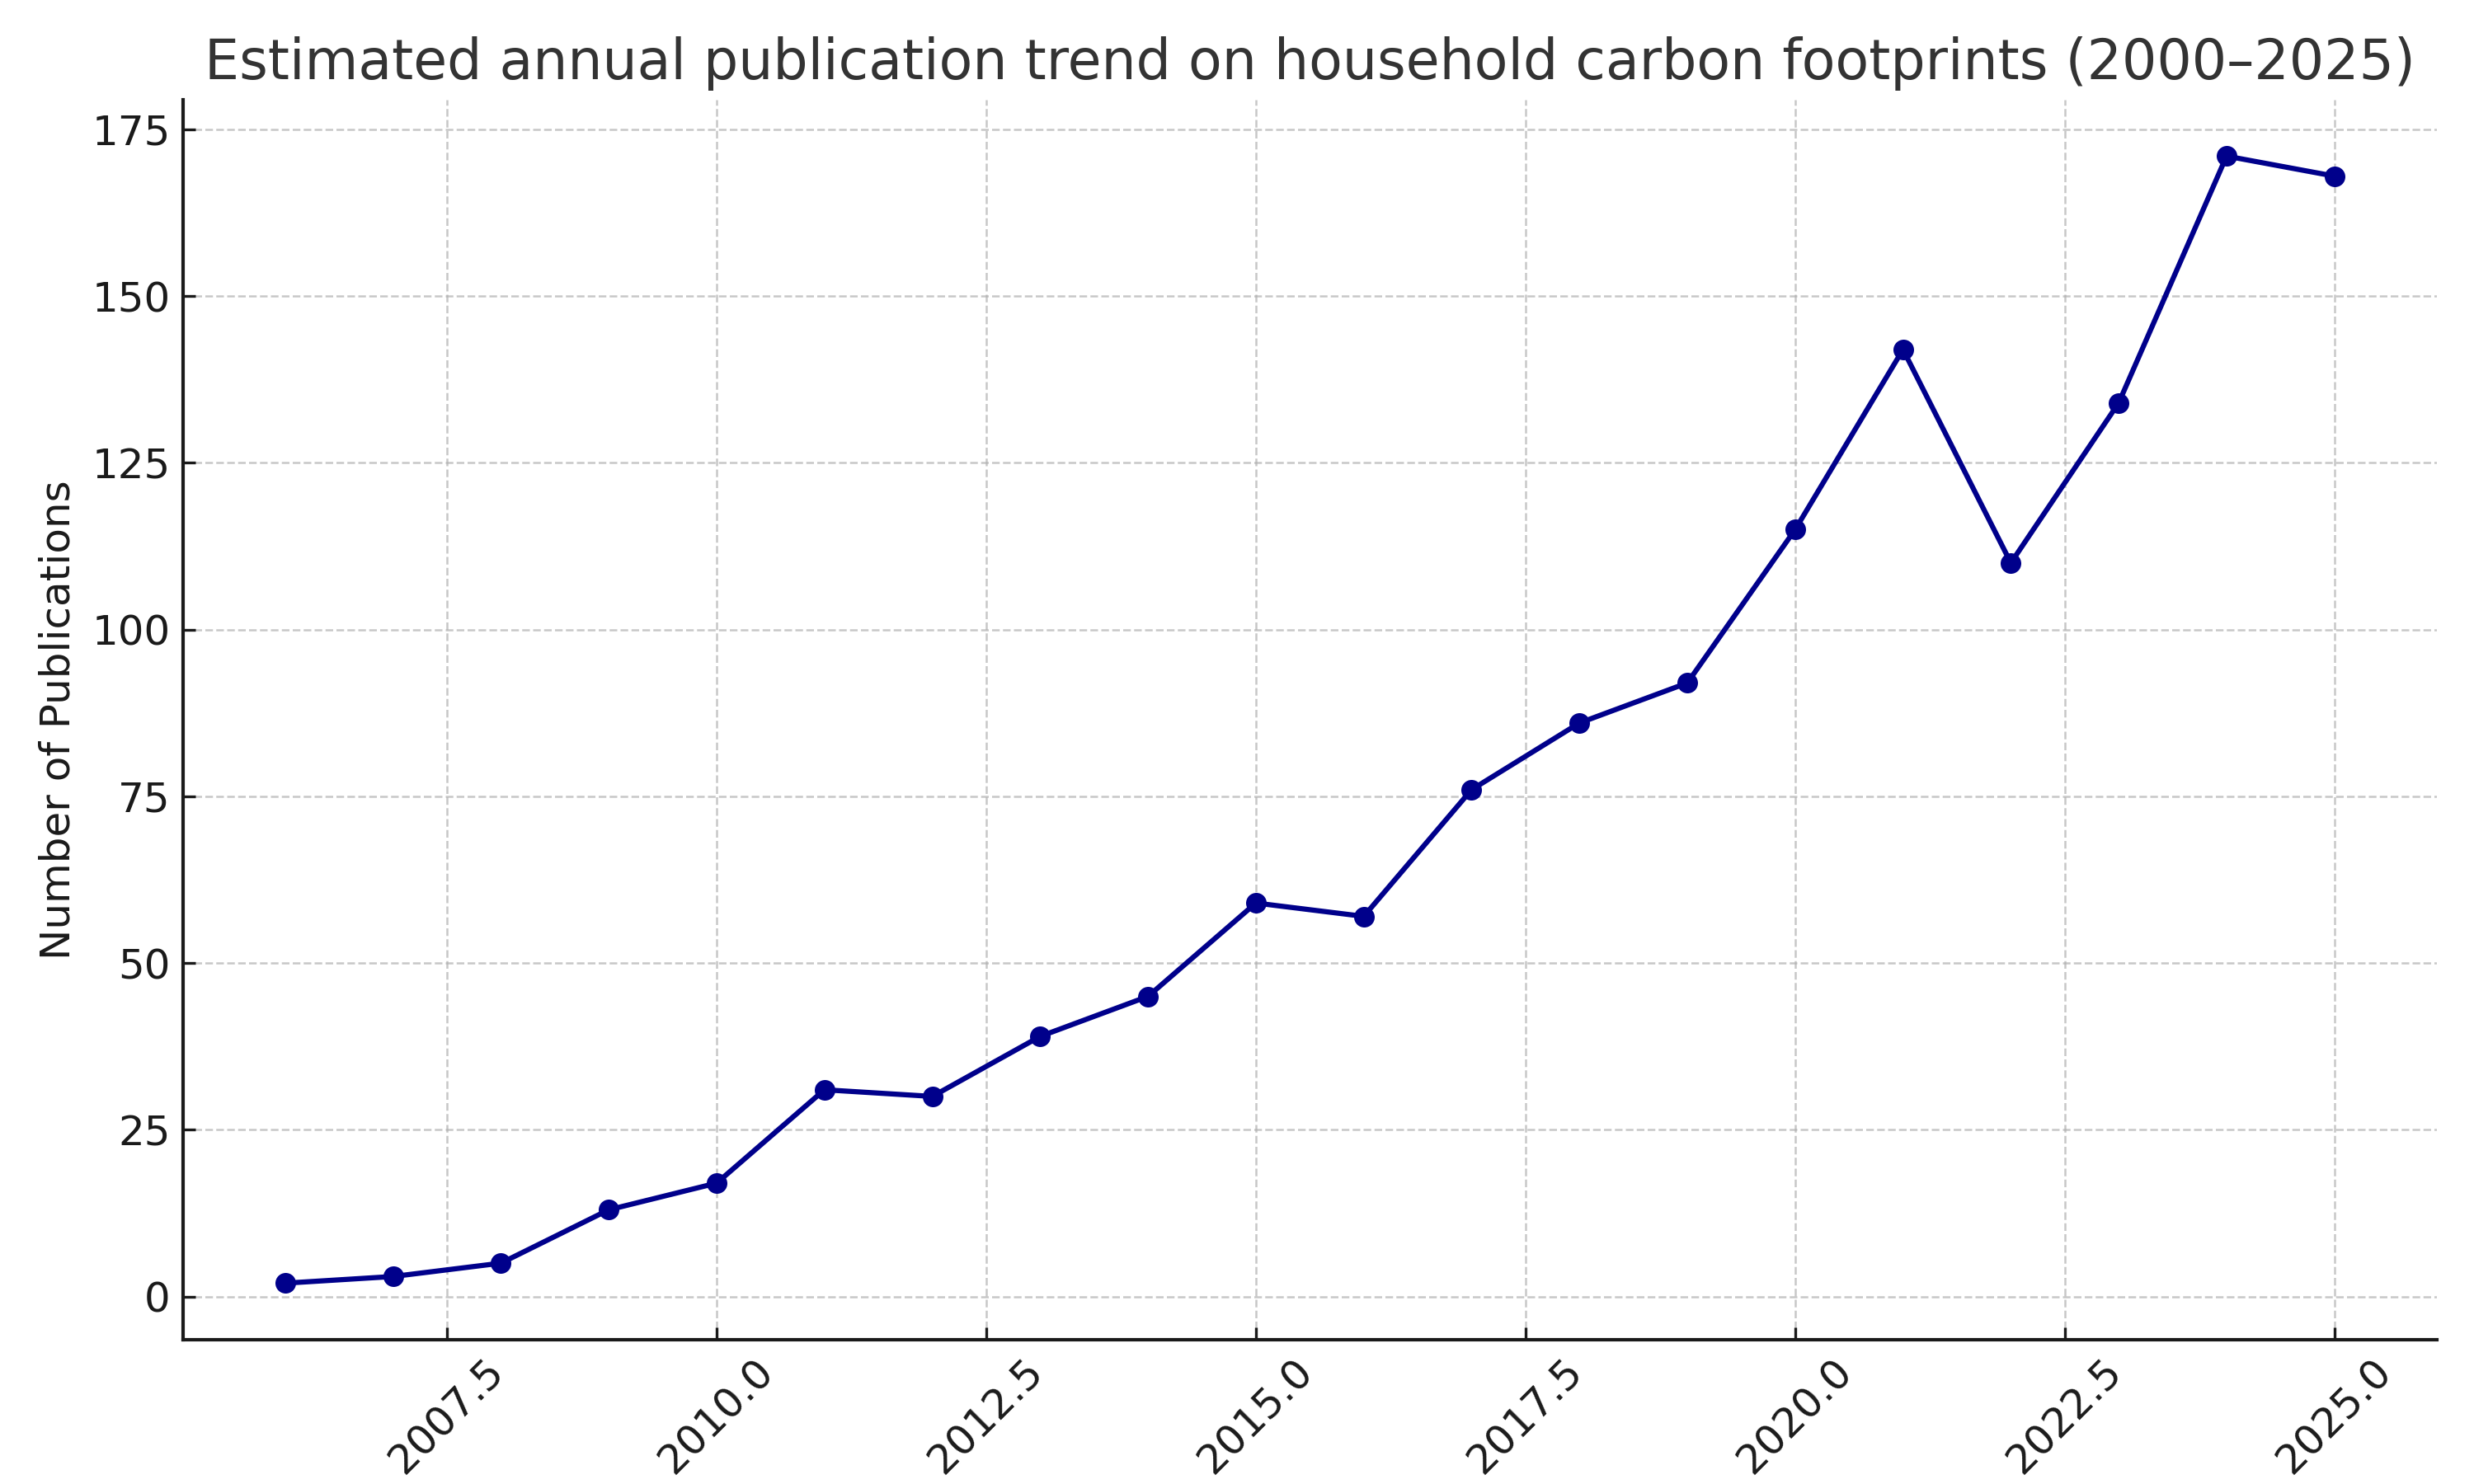
\includegraphics[width=0.85\textwidth]{publication_trend_darkblue_estimated2025.png}
    \caption{Estimated annual publication trend on household carbon footprints (2000–2025). The 2025 value is a linear extrapolation based on mid-year data.}
\end{figure}

\begin{figure}[htbp]
    \centering
    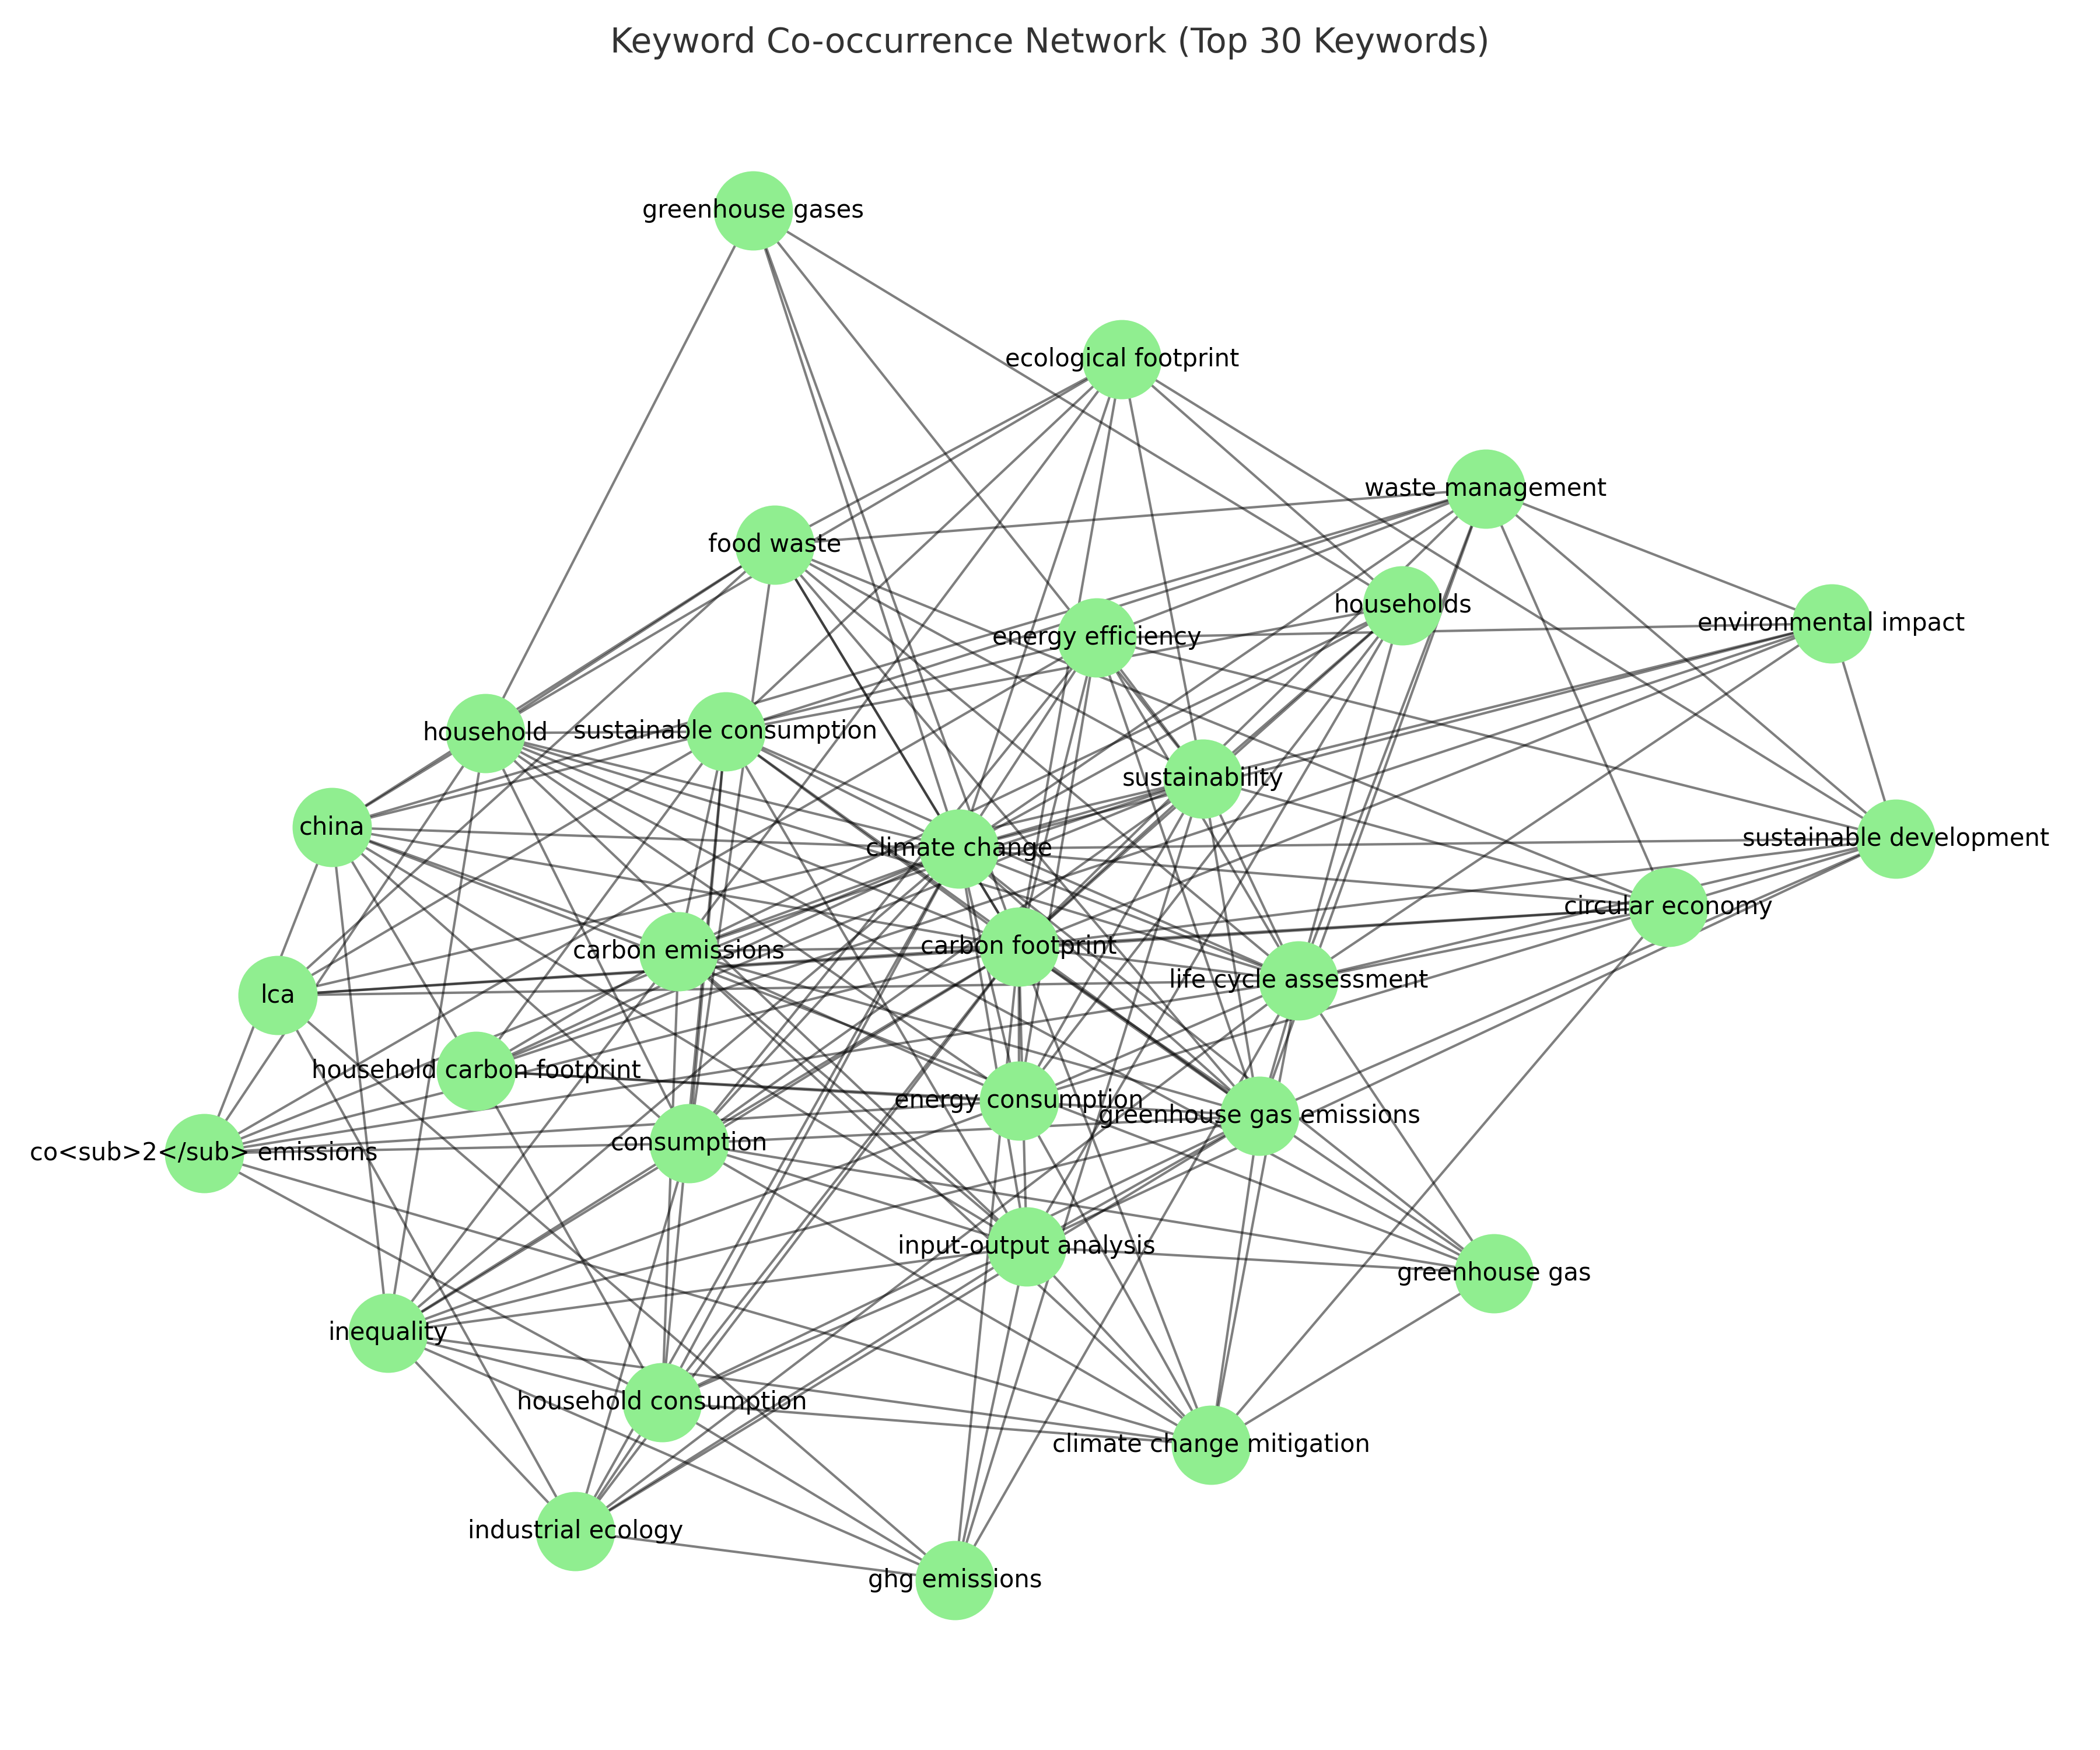
\includegraphics[width=0.85\textwidth]{keyword_cooccurrence.png}
    \caption{Keyword co-occurrence network for the 30 most frequently used terms in household carbon footprint literature (2000–2025).}
\end{figure}

The estimation of household carbon footprints in this literature review has relied on a range of methods, each grounded in distinct assumptions about attribution, causality, and system boundaries. The Greenhouse Gas (GHG) Protocol developed by the World Resources Institute and the World Business Council for Sustainable Development (WRI and WBCSD, 2004) remains a foundational standard for measuring direct (Scope 1), energy-related (Scope 2), and indirect (Scope 3) emissions. Its approach, based on multiplying activity data by standardized emission factors, is also formalized in the IPCC Guidelines (IPCC, 2019), and has been applied in national inventories and corporate disclosures. Weber and Matthews (2008) adapted this framework for household-level analysis in the United States, producing emission estimates based on household expenditure data. Life cycle assessment (LCA) methods represent a more detailed approach, estimating cradle-to-grave emissions across all stages of a product's life. Studies such as Guinée (2011) and Steubing et al. (2022) apply LCA to household consumption, though the method often requires high-resolution data and faces boundary truncation issues. Input-output analysis (IOA), especially in its environmentally extended form (EEIOA), has enabled system-wide footprinting by linking household expenditures to upstream emissions. Baiocchi and Minx (2010) applied EEIOA to compare household footprints across Europe, while Wiedmann et al. (2009) introduced a theoretical foundation for multi-regional models. Ivanova et al. (2016) added a spatial inequality perspective across global households.\footnote{Hybrid models have sought to combine the detail of LCA with the coverage of IOA, as in Sonesson et al. (2017) for food systems and in Chard (2024) and Hasegawa et al. (2021) for investment-based emissions.}A more recent contribution by Hakenes and Schliephake (2024) formalizes household carbon footprint estimation within a general equilibrium framework by endogenizing consumption and investment decisions. Their model captures the transmission of emissions through relative price changes and sectoral reallocation, enabling a behaviorally responsive and causally consistent attribution of both direct and indirect household responsibility.

Despite substantial methodological innovation, critical gaps remain in the literature on household carbon footprint estimation. Emission factor models and life cycle assessment frameworks often treat household preferences and market interactions as exogenous or fixed, limiting their ability to simulate policy-induced behavioral change (Guinée 2011; IPCC 2019). Environmentally extended input-output models, while capable of tracing upstream emissions across global supply chains, typically rely on static technical coefficients and lack behavioral realism in their representation of household decision-making\footnote{See Wiedmann et al. 2009; Ivanova et al. 2016}. Hybrid approaches\footnote{See footnote 6} improve sectoral resolution but generally do not incorporate the endogeneity of prices, income effects, or inter-household spillovers. Moreover, recent studies that examine the carbon intensity of investment portfolios have expanded the scope of household responsibility (Hasegawa et al. 2021), yet often do so in partial equilibrium settings that abstract from feedback effects across markets. The model introduced by Hakenes and Schliephake (2024) addresses many of these limitations by embedding household consumption and investment behavior within a general equilibrium framework. This approach allows for the propagation of individual decisions through price mechanisms and sectoral reallocation, thereby capturing indirect responsibility in a structurally consistent way.

Taken together, the reviewed literature offers a broad but fragmented understanding of household carbon responsibility. While methodological advances have enhanced precision and coverage, questions remain about the causal validity and policy relevance of different approaches. This paper contributes by systematically comparing four major estimation methods—emission factor accounting, life cycle assessment, input-output analysis, and the general equilibrium model proposed by Hakenes and Schliephake—through empirical illustrations and critical evaluation. Beyond methodological comparison, the analysis is motivated by a broader concern: that household-level behavioral change, while symbolically important, offers limited mitigation potential without structural reform on the supply side. As energy and food demands grow with population pressures, the study advocates for shifting the focus of policy design toward upstream interventions in production systems rather than overemphasizing downstream consumption.

\section{Methodology}

This study adopts a comparative and model-based approach to assess the carbon footprints attributable to household consumption and investment behavior. The methodology progresses in three stages: (i) the development of a conceptual framework to analyze carbon accounting methods, (ii) the empirical illustration of four representative models using synthetic household data, and (iii) a comparative evaluation of the normative implications and attribution of responsibility across models. 

The four models considered are: the Greenhouse Gas Protocol (GHGP), Life Cycle Assessment (LCA), Environmentally Extended Input–Output (EEIO) analysis, and the general equilibrium model developed by Hakenes and Schliephake (2024). These methods differ in their conceptual orientation: GHGP, LCA, and EEIO provide descriptive or accounting-based estimates of emissions tied to observed activities, while the HS model is consequentialist, modeling the systemic effects of household behavior through market mechanisms. 

Each model is implemented using data sources that reflect its underlying methodological logic and disciplinary context. The Greenhouse Gas Protocol (GHGP) model combines household consumption expenditure data for Spain in 2022 from Instituto Nacional de Estadística (INE) with emission factors from IPCC guidelines and national energy agencies, enabling scope-based estimation across direct, energy-related, and value chain emissions. The life cycle assessment (LCA) model is presented conceptually rather than empirically, drawing on studies such as Guinée (2011), Peng (2021), and Steubing et al. (2022), which illustrate cradle-to-grave emissions accounting for household goods and services. The environmentally extended input--output (EEIO) model uses household expenditure data from \textit{Eurostat} and spend-based emission factors from \textit{Climatiq.io} (sourced from \textit{EXIOBASE}), covering France, Spain, and Germany for the year 2021. Finally, the general equilibrium model by Hakenes and Schliephake (2024) is implemented using U.S. agricultural sector data, combining wheat production statistics with sectoral emissions from the \textit{USDA} and \textit{FAO} to simulate investor and consumer behavior in a closed economic system. 

The illustrations are intended to highlight how different approaches assign responsibility to households, causality of emissions and reflect varying degrees of abstraction. Rather than pursuing numerical comparability, the analysis foregrounds interpretive contrasts—examining how each method conceptualizes the role of households within the broader carbon economy. These methodological divergences form the basis for a normative analysis of climate responsibility, leading to a critical evaluation of the relevance and fairness of household-targeted policy interventions.

\section{The GHG Protocol}
The Greenhouse Gas (GHG) Protocol is a globally recognized standard for accounting and reporting greenhouse gas emissions. Developed in the late 1990s through a collaboration between the World Resources Institute (WRI) and the World Business Council for Sustainable Development (WBCSD), the GHG Protocol was officially launched in 2001 with the primary aim of providing a consistent and comprehensive framework for emissions accounting across corporate and public sectors. Over the years, its importance has grown significantly, with subsequent expansions such as the development of the GHG Protocol Scope 3 Standard in 2011, which broadened the accounting boundary to include indirect emissions across a company’s value chain. 

The principal reason for employing the GHG Protocol in household-level emissions analysis lies in its capacity to provide a standardized and granular approach to calculating emissions across different dimensions of behavior. It allows for a full inventory of climate impacts arising from everyday life—from fueling a car to investing in equity portfolios. Additionally, the protocol facilitates benchmarking across time and geography, making it possible to compare the carbon intensities of different households or regions. This is particularly valuable for policy-making, where a reliable basis for comparison is needed to design effective incentives, taxes, or subsidy programs aimed at reducing emissions. Moreover, with the rise of ESG (Environmental, Social, and Governance) investing, households are increasingly motivated to assess not only their consumption patterns but also the environmental implications of their financial choices. The GHG Protocol's inclusion of Scope 3 investment-related emissions is thus particularly timely and relevant.

\subsection{Methodological Framework of the GHG Protocol}
The mathematical formulation under the GHG Protocol for calculating a household’s carbon footprint begins with the aggregation of emissions across three main scopes of emissions. The total carbon footprint of a household is expressed as:

\begin{equation}
CF_{\text{household}} = E_{\text{Scope 1}} + E_{\text{Scope 2}} + E_{\text{Scope 3}}
\end{equation}

Each of these components is calculated based on the product of activity data and corresponding emission factors. For Scope 1, this includes the quantity of fuel combusted in household-controlled devices or vehicles, multiplied by the fuel-specific emission factor. Scope 2 emissions are determined by multiplying electricity or district heating usage by grid-specific emission factors. Scope 3 is more complex and can be further disaggregated into emissions from the consumption of goods and services, and emissions from household investments. For the consumption subcategory, expenditures are multiplied by lifecycle emission factors derived from environmentally extended input-output models or product-level lifecycle assessments. For investment-based emissions, the monetary value of investments is multiplied by portfolio-weighted emission intensities of the respective industries.

To demonstrate how the GHG Protocol method can be applied in practice, the following section uses household consumption data from Spain for the year 2022 as an illustrative case. Based on this calculation, the total household carbon footprint is estimated at approximately 11,828 kg CO$_2$e per year, with indirect emissions accounting for the largest share, which reflects a pattern widely documented in studies of household carbon footprints in high-income countries (Hertwich and Peters, 2009; Ivanova et al., 2016). 
\subsection{Application of the GHG Protocol to Spanish Household Data (2022)}

As an empirical demonstration, the GHG Protocol framework is applied to household expenditure data for Spain in 2022 to illustrate the distribution of emissions across Scopes 1, 2, and 3. The data, sourced from the \textit{Instituto Nacional de Estadística (INE)}, report an average annual household expenditure of €31,568, disaggregated by \textit{COICOP}\footnote{COICOP refers to the Classification of Individual Consumption According to Purpose, a UN standard for categorizing household consumption expenditures. See United Nations Statistics Division (2018).} classification. Spending is allocated across major categories such as housing and energy (32.4\%), food and beverages (16.0\%), and transport (12.0\%), with growing shares in services such as restaurants and hotels. This categorical breakdown enables the assignment of emission factors to each expenditure type. A full summary is presented in Table A4 of Appendix A.



Scope 1 emissions are derived from the direct combustion of fossil fuels by households, primarily through private vehicle use and residential heating. Energy consumption data, expressed in gigajoules (GJ) per capita, are sourced from the Instituto Nacional de Estadística (INE).\footnote{INE (2022), "Encuesta de Presupuestos Familiares," and energy balance data.} Emission factors are drawn from DEFRA and IPCC guidelines, with petrol estimated at 73.3 kg CO\textsubscript{2}e/GJ and natural gas at 56.1 kg CO\textsubscript{2}e/GJ. The corresponding calculations are presented in Table 1. Scope 2 emissions refer to indirect emissions associated with the consumption of purchased energy, primarily electricity and district heating, generated externally. In 2022, the average Spanish household consumed approximately 8.96 GJ of heating and cooling energy, with the national electricity grid's emission factor estimated at 92.6 kg CO\textsubscript{2}e per GJ, see Table 2 for the calculations.

% Ensure \usepackage{graphicx} is in your preamble

\begin{table}[h]
\centering
\captionsetup{justification=raggedright,singlelinecheck=false} 
\caption{\small Direct Emissions from Household Energy and Transport (Scope 1)}\label{tab:scope1}
\resizebox{\textwidth}{!}{%
\begin{tabular}{lccc}
\toprule
\textbf{Energy Source} & \textbf{Consumption (GJ/hab)} & \textbf{Emission Factor (kg CO$_2$e/GJ)} & \textbf{Emissions (kg CO$_2$e)} \\
\midrule
Natural Gas (Transport) & 0.04 & 56.1 & 2.24 \\
Petrol (Transport)      & 14.44 & 73.3 & 1058.45 \\
Natural Gas (Heating)   & 0.73 & 56.1 & 40.95 \\
Petrol (Other)          & 0.18 & 73.3 & 13.19 \\
\midrule
\textbf{Total}          &       &       & \textbf{1114.83} \\
\bottomrule
\end{tabular}%
}
\raggedright
\textit{\footnotesize{Source: Author's calculations based on INE (2022), DEFRA (2022), and IPCC (2019) emission factors.}}
\end{table}


\begin{table}[h]
\centering
\captionsetup{justification=raggedright,singlelinecheck=false} 
\caption{\small Indirect Emissions from Heating and Cooling (Scope 2)}\label{tab:scope2}
\resizebox{\textwidth}{!}{%
\begin{tabular}{lccc}
\toprule
\textbf{Energy Source} & \textbf{Consumption (GJ/hab)} & \textbf{Emission Factor (kg CO$_2$e/GJ)} & \textbf{Emissions (kg CO$_2$e)} \\
\midrule
Heating/Cooling Energy & 8.96 & 92.6 & 829.70 \\
\midrule
\textbf{Total} & & & \textbf{829.70} \\
\bottomrule
\end{tabular}%
}
\raggedright
\textit{\footnotesize{Source: Author's calculations based on INE (2022), DEFRA (2022), and IPCC (2019) emission factors.}}
\end{table}

Scope 3 emissions represent the most extensive component of the household carbon footprint, capturing the indirect environmental impacts associated with consumption. These emissions encompass the carbon embedded in food, manufactured goods, services, and transport-related infrastructure. Each expenditure category is assigned a specific emission factor, derived from lifecycle assessment data, and multiplied by corresponding household spending. For instance, food consumption carries an average emission factor of 0.50 kg CO\textsubscript{2}e per euro, accounting for agricultural production, processing, and distribution. Clothing is assigned a lower factor of 0.25 kg CO\textsubscript{2}e/€, while restaurant services, due to their higher energy intensity, are estimated at 0.40 kg CO\textsubscript{2}e/€. Detailed category-level results for Scope 3 are shown in Table 3.
% Make sure you have \usepackage{booktabs} and \usepackage{graphicx} in your preamble

\begin{table}[h]
\centering
\captionsetup{justification=raggedright,singlelinecheck=false} 
\caption{\small Consumption-Based Emissions (Scope 3)}\label{tab:scope3}
\resizebox{\textwidth}{!}{%
\begin{tabular}{lccc}
\toprule
\textbf{Category} & \textbf{Expenditure (€)} & \textbf{Emission Factor (kg CO$_2$e/€)} & \textbf{Emissions (kg CO$_2$e)} \\
\midrule
Food and non-alcoholic beverages & 5,050 & 0.50 & 2,525.00 \\
Alcoholic beverages and tobacco  &   481 & 0.30 &   144.30 \\
Clothing and footwear            & 1,232 & 0.25 &   308.00 \\
Housing and utilities            &10,243 & 0.25 & 2,560.75 \\
Furnishings                      & 1,296 & 0.30 &   388.80 \\
Health                           & 1,228 & 0.20 &   245.60 \\
Transport services               & 3,794 & 0.30 & 1,138.20 \\
Communications                   &   925 & 0.15 &   138.75 \\
Recreation                       & 1,534 & 0.35 &   536.90 \\
Education                        &   468 & 0.10 &    46.80 \\
Restaurants and hotels           & 2,953 & 0.40 & 1,181.20 \\
Miscellaneous goods and services & 2,364 & 0.30 &   709.20 \\
\midrule
\textbf{Total}                   &        &       & \textbf{9,883.55} \\
\bottomrule
\end{tabular}%
}
\raggedright
\textit{\footnotesize{Source: Author's calculations based on INE (2022), DEFRA (2022), and IPCC (2019) emission factors.}}
\end{table}

Summing all three scopes, the total annual carbon footprint of a Spanish household in 2022 is estimated at 11,828.08 kg CO\textsubscript{2}e. While Scope 1 and Scope 2 together account for less than 20 \% of the total footprint, largely reflecting fuel use for transport and home energy consumption, Scope 3 alone contributes over four-fifths of total emissions.\footnote{see Table 4} This pattern emphasizes that even households with modest direct energy use can maintain high overall footprints due to the embedded emissions in everyday consumption, pointing to the critical importance of addressing upstream emissions in climate policy.
% Make sure \usepackage{booktabs} is in your preamble

\begin{table}[h]
  \captionsetup{justification=raggedright,singlelinecheck=false} 
\caption{\small Total Household Carbon Footprint by Emission Scopes}\label{tab:total_emissions}
\begin{tabular}{lcccc}
\toprule
 & \small \textbf{Scope 1} & \small \textbf{Scope 2} & \small \textbf{Scope 3} & \small \textbf{Total} \\
\midrule
\small \textbf{Emissions (kg CO$_2$e)} & \small 1,114.83 & \small 829.70 & \small 9,883.55 & \small 11,828.08 \\
 \bottomrule
\end{tabular}

\raggedright
\textit{\footnotesize{Source: Author's calculations based on INE (2022), DEFRA (2022), and IPCC (2019) emission factors.}}
\end{table}


\subsection{Limitations of the GHG Protocol}

Although widely adopted, the GHG Protocol framework exhibits key limitations when applied to household carbon footprint estimation. Its reliance on average emission factors and static expenditure profiles restricts its capacity to reflect behavioral responses to price signals or policy changes. As evidenced in the Spanish household illustration, Scope 3 emissions constitute the bulk of the footprint, yet the model lacks sensitivity to substitution effects, rebound dynamics, and income elasticity of demand (Hertwich and Peters (2009); Munksgaard et al. (2000)). Furthermore, the use of nationally aggregated emission factors masks regional variability in electricity generation, heating fuels, and consumption infrastructure, potentially distorting footprint estimates in subnational contexts (Lenzen et al. (2004); Wiedmann (2009)).

Enhancing the model with regionally disaggregated data and behavioral elasticities would improve its diagnostic and predictive utility. Incorporating time-series data would further allow for longitudinal assessments of household responses to mitigation policies. Finally, expanding the accounting boundary to include complementary sustainability metrics, such as water use, material intensity, and land footprint, would allow for a more comprehensive assessment of household environmental impacts beyond carbon alone (Wiedmann \& Minx, 2008).

\section{Life Cycle Assessment (LCA) Method}
The LCA method calculates emissions throughout the entire life cycle of a product or service, from production to disposal. This model captures emissions from every stage of the supply chain and provides a comprehensive assessment of indirect emissions.

The carbon footprint for a single industry using the LCA approach is:
\begin{equation}
   fp_h = q_h \cdot \text{LCA}_j 
\end{equation}

where \(q_h\) is the quantity consumed by household \(h\), and \(\text{LCA}_j\) represents the life cycle emissions per unit in industry \(j\).


\subsection{Methodology for Household Carbon Footprint Calculation based on LCA approach}
This section adapts the framework developed by Peng et al. (2021) to estimate household carbon footprints by combining complementary life cycle assessment (LCA) techniques. Aligned with principles outlined in Guinée (2011) and comparative reviews such as Matthews et al. (2008) and Steubing et al. (2022), the approach quantifies both direct and embodied greenhouse gas (GHG) emissions, together with net carbon sequestration linked to household-level activities.

The methodology integrates three LCA variants to address the system boundary limitations inherent in partial assessments: (1) Process-based LCA is applied to quantify emissions from agricultural operations and livestock production, capturing emissions embedded in material inputs and field-level activities; (2) Input–Output LCA extends the boundary to indirect emissions embedded in household consumption of energy, food, housing, and transport, using environmentally extended input–output (EEIO) tables (Weber and Matthews, 2008); (3) Hybrid LCA bridges both levels by combining process inventory detail with macroeconomic input–output linkages, reducing truncation errors and capturing carbon flows related to afforestation, durable goods, and other land-use changes (Crawford et al., 2018; Shen et al., 2023).

Following Peng et al. (2021), the model distinguishes five core domains: direct energy use, short-lived and durable consumption, household agriculture, afforestation, and livestock management. Activity-specific emissions are parameterized using survey-derived data and regionally adjusted emission factors in accordance with IPCC (2019) guidelines. This combined accounting framework quantifies net household carbon flows as the balance of annual GHG emissions and sequestration within a unified system boundary:

\begin{equation}
CF_i = \sum_{n} E_{in} + \sum_{m} S_{im}
\end{equation}
where $CF_i$ represents the Carbon footprint of household $i$, $E_{in}$ is the annual carbon emissions of household $i$ in category $n$ and $S_{im}$ is the annual carbon sequestration of household $i$ in category $m$. This disaggregated yet integrated structure provides the basis for the following activity-specific equations, which formally express how annual household emissions and sequestration are calculated within each functional domain.

\subsection{Carbon Emissions from Direct Energy Consumption}
The emissions from household direct energy use are estimated by multiplying the quantity of fuel consumed by its corresponding emission factor. For each household ii, the total emissions attributable to direct fuel combustion are calculated as:
\begin{equation}
E_{id} = \sum_d (F_{id} \cdot EF_d)
\end{equation}
where $F_{id}$ denotes the annual consumption of household $i$  for fuel type $d$. The fuel-specific emission factor $E_{id}$ combines oxidation efficiency, fuel composition, and calorific value, consistent with IPCC (2019) guidelines:
\begin{equation}
EF_d = OX_d \cdot \left(C_{o,d} \cdot \frac{12}{44} + C_{h,d} \cdot \frac{12}{16}\right) \cdot H_d \cdot 10^{-9}
\end{equation}
Here, $OX_d$ represents the oxidation efficiency, typically assumed to be 100\% for complete combustion; $C_{o,d}$ and $C_{h,d}$ are the fuel-specific emission coefficients for CO$_2$ and CH$_4$, respectively; and $H_d$ denotes the net calorific value of the fuel. The conversion factors ensure that carbon content is expressed in consistent units of tonnes CO$_2$ equivalent per unit of fuel input.

\subsection{Carbon Emissions from Living Consumption}

Emissions attributable to household consumption of goods and services are divided into two categories: short-lived products and durable consumer goods. The total annual emissions from short-lived consumption are given by:

\begin{equation}
E_{if} = \sum_f (EF_f \cdot C_{if})
\end{equation}

where $E_{if}$ denotes the annual carbon emissions from short-lived good $f$, $C_{if}$ is the quantity of product $f$ consumed by household $i$, and $EF_f$ is its corresponding life cycle emission factor. For durable consumer products, the embodied emissions are amortized over the product's expected service life to obtain an annualized footprint:

\begin{equation}
E_{ij} = \sum_j \frac{(EF_j \cdot C_{ij})}{L_j}
\end{equation}

Here, $E_{ij}$ represents the annual emissions associated with durable product $j$, $C_{ij}$ is the total quantity purchased, $EF_j$ is the relevant life cycle emission factor, and $L_j$ is the product’s average lifetime (in years). This treatment ensures that emissions embedded in capital household goods are allocated proportionally across their period of use, consistent with standard LCA accounting conventions.


\subsection{Carbon Footprint in Agricultural Activities}

Emissions and sequestration associated with household-level agricultural production are accounted for through inputs, on-site operations, and net biomass growth. The total annual carbon footprint from agricultural activities for household $i$ is calculated as:

\begin{equation}
CF_{ia} = \sum_a (EF_a \cdot M_{ia}) + \sum_t (EF_t \cdot FS_{ia}) + \sum_v (B_v \cdot 0.475)
\end{equation}

Here, $CF_{ia}$ denotes the net carbon impact of agricultural activities. $M_{ia}$ represents the quantity of material input $a$ (such as fertilizers or pesticides) applied by household $i$, with an associated emission factor $EF_a$. The second term accounts for emissions from field operations, where $FS_{ia}$ is the cultivated field size and $EF_t$ is the emission factor per unit area for operation $t$ (e.g., tillage, irrigation). The final term reflects the carbon sequestered in above-ground biomass, with $B_v$ indicating the dry biomass yield for crop or vegetation type $v$, multiplied by a standard carbon content coefficient of 47.5\% (IPCC default for plant biomass).


\subsection{Carbon Sequestration from Afforestation}

Carbon sequestration through household-level afforestation is estimated based on the area of land dedicated to tree planting and the average carbon stock of the tree species established. The annual sequestration from afforestation for household $i$ is given by:

\begin{equation}
S_{iaf} = FS_{iaf} \cdot CS_{\text{citrus}}
\end{equation}

In this expression, $S_{iaf}$ represents the amount of carbon sequestered through afforestation activities, $FS_{iaf}$ denotes the field size (in hectares) allocated for tree planting by household $i$, and $CS_{\text{citrus}}$ is the mean carbon stock per unit area for citrus trees or other comparable species. The carbon stock factor reflects the average annual carbon uptake, accounting for biomass accumulation under local growth conditions.


\subsection{Carbon Emissions from Livestock Raising}

Emissions from household livestock activities include fodder production, enteric fermentation, and manure management. The total annual emissions from livestock raising for household $i$ are calculated as:

\begin{equation}
E_{il} = \sum_f (EF_{if} \cdot F_{if}) + \sum_l (EF_{il} \cdot N_{il})
\end{equation}

In this formulation, $E_{il}$ represents the total carbon emissions attributable to livestock-related activities. $F_{if}$ denotes the annual quantity of fodder consumed by livestock, multiplied by the corresponding emission factor $EF_{if}$ to account for upstream impacts of fodder cultivation and transport. The second term captures direct emissions from livestock, where $N_{il}$ is the number of animals of type $l$ and $EF_{il}$ is the per-animal emission factor, which includes methane emissions from enteric fermentation and nitrous oxide from manure management.



\subsection{Aggregate Formula for Household Carbon Footprint}

The total household carbon footprint ($CF_{\text{total}}$) aggregates emissions and sequestration from direct energy use, living consumption, agricultural production, afforestation, and livestock raising, as specified in Equations (4) to (10).

\begin{align}
CF_{\text{total}} = & \underbrace{\sum_d \left(F_{id} \cdot EF_d\right)}_{\text{Direct energy}} + 
\underbrace{\sum_f \left(EF_f \cdot C_{if}\right) + \sum_j \frac{\left(EF_j \cdot C_{ij}\right)}{L_j}}_{\text{Living consumption}} \nonumber \\
& + \underbrace{\sum_a \left(EF_a \cdot M_{ia}\right) + \sum_t \left(EF_t \cdot FS_{ia}\right) + \sum_v \left(B_v \cdot 0.475\right)}_{\text{Agriculture}} \nonumber \\
& - \underbrace{\sum_{iaf} \left(FS_{iaf} \cdot CS_{\text{citrus}}\right)}_{\text{Afforestation}} +
\underbrace{\sum_f \left(EF_{if} \cdot F_{if}\right) + \sum_l \left(EF_{il} \cdot N_{il}\right)}_{\text{Livestock}}.
\label{eq:aggregate}
\end{align}

By integrating disaggregated activity data with region-specific emission factors, this aggregate formulation is a consistent representation of the net annual GHG balance at the household level, consistent with best practices in household carbon accounting (Ivanova et al., 2016; Dubois et al., 2019). 

Beyond its measurement function, this structure highlights how household decisions on energy use, consumption patterns, and land management jointly influence emissions outcomes (Hertwich and Peters, 2009). Such clarity enables scenario analysis of behavioral shifts and technological choices, informing targeted interventions like carbon price adjustments, renewable energy adoption incentives, or compensation for sequestration through land-based measures (Rogelj et al., 2018; Steubing et al., 2022). As shown in recent household-level studies, aligning micro-level incentives with broader climate objectives is essential to internalize externalities and realize cost-effective emission reductions (Wiedmann et al., 2020).

\subsection{Household Emissions Breakdown under LCA}

An integrated life cycle assessment (LCA) illustration clarifies how the total household carbon footprint, as defined by Equations (4) to (10), is distributed across major activity domains and is illustrated in Figure 3. Drawing on estimates from Peng et al.\ (2021), Sala et al.\ (2014), and Matthews et al.\ (2008), direct household energy use, including heating fuels and private vehicle fuels, accounts for approximately 20\% to 30\% of total greenhouse gas emissions. Living consumption, which covers short-lived goods, food purchases, and services, represents the largest share at about 50\% to 60\%. Durable goods, including household appliances and furniture, add an additional 5\% to 10\% of total emissions when annualized, showing the relevance of product lifespan and embedded material flows. 

Together, this evidence shows that focusing only on direct household fuel use underestimates the total climate impact of residential lifestyles because indirect emissions embedded in goods and services account for most impacts, as discussed by Hertwich and Peters (2009). A comprehensive, activity-based LCA offers a more realistic basis for identifying mitigation options such as improving building energy performance, extending product lifespans, sourcing materials more sustainably, and investing in land-based carbon sequestration. This broader perspective supports the development of household-level strategies that address systemic drivers of emissions rather than isolating individual consumption categories.


\begin{figure}[h]
\centering
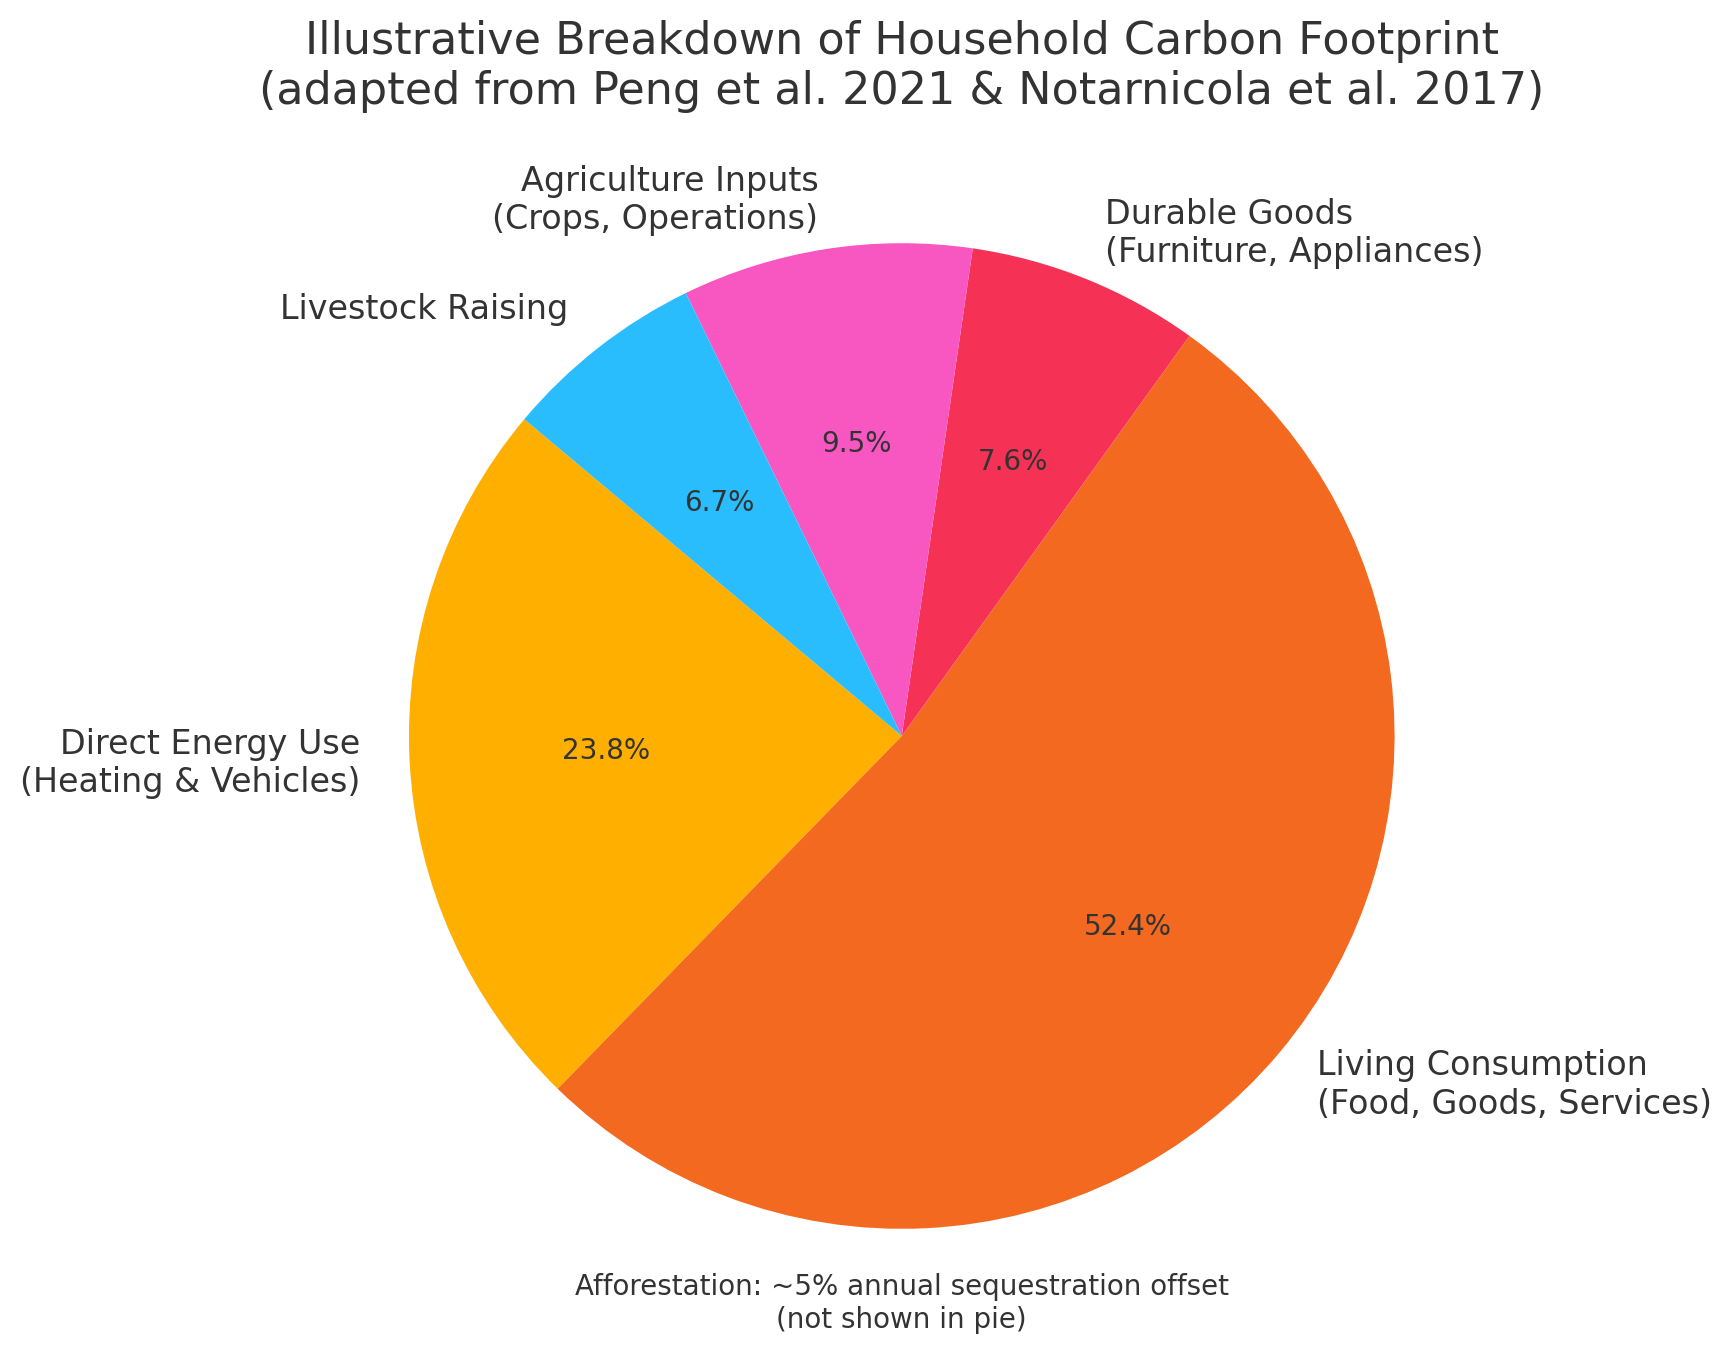
\includegraphics[width=0.8\linewidth]{LCA_pie.png}
\small \caption{Relative contribution of household activities to carbon footprint based on an integrated LCA approach. Findings are adapted from Peng et al.\ (2021), Notarnicola et al.\ (2017), and Matthews et al.\ (2008).}
\end{figure}

\section{Input–Output Model and Carbon Footprint Estimation}
The environmentally extended Input-Output (EEIO) framework provides a macroeconomic approach for quantifying household carbon footprints by tracing both direct and upstream greenhouse gas (GHG) emissions embedded in goods and services. 

\subsection{Leontief Input–Output Framework}

We begin with the standard Leontief system, where total output \( \mathbf{X} \) is the sum of intermediate input requirements and final demand:

\begin{equation}
\mathbf{X} = \mathbf{A} \mathbf{X} + \mathbf{F}.
\end{equation}

Solving for total output yields the fundamental input–output identity:

\begin{equation}
\mathbf{X} = {(\mathbf{I} - \mathbf{A})}^{-1} \mathbf{F}.
\end{equation}

Here, \( \mathbf{A} \) is the technical coefficient matrix, \( \mathbf{F} \) is the vector of household final demand, and \( {(\mathbf{I} - \mathbf{A})}^{-1} \) is the Leontief inverse, which accounts for the total production required (both direct and indirect) to satisfy final demand.

\subsection{Technical Coefficient Matrix}

Each element \( A_{ij} \) of the matrix \( \mathbf{A} \) is defined as:

\begin{equation}
A_{ij} = \frac{z_{ij}}{x_j},
\end{equation}

where \( z_{ij} \) denotes the monetary value of inputs from sector \( i \) to sector \( j \), and \( x_j \) is the total output of sector \( j \). The matrix \( \mathbf{A} \) reflects the technological input structure of the economy.

\subsection{Stability of the Leontief Inverse}

The Leontief inverse \( {(\mathbf{I} - \mathbf{A})}^{-1} \) exists and is finite if the matrix \( \mathbf{A} \) satisfies the stability condition \( \rho(\mathbf{A}) < 1 \), where \( \rho(\cdot) \) denotes the spectral radius (i.e., the largest absolute eigenvalue). This condition ensures that the production system is productive and does not require infinite inputs. In applied input--output tables, a sufficient (but not necessary) condition is that the column sums of \( \mathbf{A} \) are each less than one:
\[
\sum_i A_{ij} < 1 \quad \text{for all } j.
\]
This implies that each sector uses less than one unit of intermediate input to produce one unit of output, a condition that is generally satisfied in empirical datasets (Miller and Blair, 2009). A numerical illustration of the stability condition, along with matrix-based examples and emission multiplier computation, is provided in Appendix B.

\subsection{Carbon Footprint Estimation via Input–Output Modelling}

The environmentally extended input–output (EEIO) model estimates household carbon footprints by applying sectoral emission intensities to the total output vector required to satisfy final demand:

\begin{equation}
\mathbf{E} = \mathbf{C} {(\mathbf{I} - \mathbf{A})}^{-1} \mathbf{F},
\end{equation}

where \( \mathbf{C} \) is the vector of direct emission intensities (e.g., kg CO\textsubscript{2}e per euro of output), and \( \mathbf{E} \) is the resulting emissions attributable to household consumption. This formulation captures both direct and upstream (supply chain) emissions associated with consumption.

\subsection{Tiered Decomposition of Household Emissions}

Following Matthews et al.~(2008) and Long et al.~(2019), the total household footprint can be analytically decomposed into three tiers:

\paragraph{Tier 1: Direct Emissions}

\begin{equation}
\mathbf{E}_1 = \mathbf{C}_d \cdot \mathbf{F}_d,
\end{equation}

where \( \mathbf{F}_d \) is household consumption of directly combusted fuels and \( \mathbf{C}_d \) is the corresponding emission intensity vector.

\paragraph{Tier 2: Indirect Energy Emissions}

\begin{equation}
\mathbf{E}_2 = \mathbf{C}_e \cdot {(\mathbf{I} - \mathbf{A})}^{-1} \cdot \mathbf{F}_e,
\end{equation}

with \( \mathbf{F}_e \) representing consumption of electricity and district heating, and \( \mathbf{C}_e \) their emission intensities.

\paragraph{Tier 3: Indirect Supply Chain Emissions}

\begin{equation}
\mathbf{E}_3 = \mathbf{C} \cdot {\left[(\mathbf{I} - \mathbf{M})(\mathbf{I} - \mathbf{A})\right]}^{-1} \cdot \left[(\mathbf{I} - \mathbf{M}) \cdot \mathbf{F} + \mathbf{EX} \right],
\end{equation}

where \( \mathbf{M} \) is a diagonal matrix of sectoral import shares, and \( \mathbf{EX} \) accounts for exports. This import-adjusted EEIO formulation ensures emissions are assigned to domestic demand (Long et al., 2019; Sheng et al., 2024).

\paragraph{Total Household Footprint.}  
Combining all tiers, the household footprint is:

\begin{equation}
    \mathbf{E}_{\text{total}} = \mathbf{E}_1 + \mathbf{E}_2 + \mathbf{E}_3.
\end{equation}

This integrated EEIO framework mitigates truncation and boundary errors typical of process-based LCA, capturing the full feedback loops of modern economies (Matthews et al., 2008; Steubing et al., 2022).


\subsection{Illustrative Application of the Input-Output Model}

In this illustration, pre-calculated environmentally extended emission intensities (kg CO$_{2}$e per euro spent) are applied to household consumption data for France, Spain, and Germany for 2021. These intensities represent the aggregated effect of $\mathbf{C} {(\mathbf{I}-\mathbf{A})}^{-1}$ and are derived from the EXIOBASE multi-regional input-output (MRIO) model, as accessed via Climatiq.io.\footnote{These coefficients implicitly incorporate trade-adjusted upstream emissions, though no explicit import share matrix was applied in this illustration.} The method aligns with the tier-3 comprehensive accounting approach discussed in Matthews et al.~(2008), Long et al.~(2019), and Sheng et al.~(2024).

\subsubsection{Data and Methodology}

The Leontief inverse ${(\mathbf{I} - \mathbf{A})}^{-1}$ then expands final demand to include both direct and indirect production requirements.

\begin{equation}
  EF_i = \sum_{j} C_j L_{ji}, 
\quad \text{where} \quad 
L = {(\mathbf{I} - \mathbf{A})}^{-1}.
\end{equation}



Here, $C_j$ denotes the direct emissions intensity for producing sector $j$, and $L_{ji}$ represents the total requirements linking producing sectors $j$ and $i$. The resulting spend-based factors are published through Climatiq.io, which provides up-to-date coefficients aggregated from EXIOBASE under a permissive data license (Creative Commons Attribution-ShareAlike 4.0 International License).

To ensure numerical stability, EXIOBASE balances its input-output tables using harmonised supply-use statistics, preventing divergence in the Leontief inverse. An additional feasibility check confirms that the sum of each column in $\mathbf{A}$ remains below unity, preserving the productive structure required for invertibility.

Annual household final consumption expenditure for France, Spain, and Germany was sourced from Eurostat for the year 2021 and harmonised to euros at the average annual exchange rate. For each expenditure category $i$ and country $c$, the household carbon footprint is estimated by multiplying the national expenditure by the corresponding spend-based factor:

\begin{equation}
  E_{i,c} = F_{i,c} \times EF_i.
\end{equation}

For instance, for France, the estimated annual household spending on food and non-alcoholic beverages is approximately

\[
F_{\text{food,FR}} = 1.322 \times 10^9 \times 0.139 = 183.8 \times 10^9~\text{EUR}.
\]

Multiplying this by the category-specific factor of 0.48~kg CO$_2$e per euro yields an estimated

\[
E_{\text{food,FR}} = 183.8 \times 10^9 \times 0.48 = 88.2 \times 10^6~\text{tonnes CO}_2\text{e}.
\]

The same procedure is applied across all final demand categories and for Spain and Germany. This method follows the tier-3 EEIO approach and systematically allocates upstream supply chain emissions, providing a comprehensive perspective on the consumption-driven climate impact of households. All emission factors are listed in Appendix~A, Table~A5.

\subsubsection{Results}

Table 5 summarizes the estimated household carbon footprints for France, Spain, and Germany in 2021, derived using the environmentally extended input--output model. The full breakdown by expenditure category is reported in Appendix~A (Tables~A6--A8).

\begin{table}[h]
 \captionsetup{justification=raggedright,singlelinecheck=false} 
\caption{\small{Total estimated household carbon footprints (2021)}}
\begin{tabular}{lcc}
\toprule
\textbf\small{Country} & \textbf\small{Expenditure (bn €)} & \textbf\small{Emissions (Mt CO\textsubscript{2}e)} \\
\midrule
\small France & \small 1322.0 & \small 420.0 \\
\small Spain & \small 747.9 & \small 227.0 \\
\small Germany & \small 1794.8 & \small 545.9 \\
\bottomrule
\end{tabular}
\raggedright

\textit{\footnotesize{Source: Author's calculations based on Eurostat 2021 data on Household final consumption expenditure by purpose (COICOP 1999) and EXIOBASE (2025) emission factors.}}
\end{table}

In all three countries, the dominant drivers of household emissions are housing, food, and transport. These sectors together account for over 60\% of the footprint, reflecting the carbon intensity of residential energy use, agri-food supply chains, and private mobility. The relative magnitude and structure of results are consistent with earlier multi-regional IO studies (Matthews et al.~2008; Long et al.~2019; Sheng et al.~2024), confirming the utility of EEIO methods for policy-relevant footprint accounting.

Thus, the footprint estimates capture the sectoral and cross-country variation in household carbon intensity, illustrating the effectiveness of the EEIO approach in quantifying consumption-driven emissions at national scale.


\subsection{Comparative Assessment of LCA and EEIOA for Household Carbon Footprint Estimation}

Life cycle assessment (LCA) and environmentally extended input--output analysis (EEIOA) are both established approaches for estimating household carbon footprints but differ in system boundaries and detail. LCA quantifies emissions by summing process-based impacts across all life cycle stages, often including capital goods and infrastructure explicitly.

In this illustration, the household carbon footprint is quantified using an LCA framework adapted from Steubing et al.~(2022). The structure of the total footprint, previously defined in Equation~(11), can be re-stated as:

\begin{equation}
\text{CF}_{\text{total}} = \sum_d (F_{id} \cdot EF_d) 
+ \sum_f (C_{if} \cdot EF_f) 
+ \sum_j \left( \frac{C_{ij} \cdot EF_j}{L_j} \right)
+ \sum_a (M_{ia} \cdot EF_a)
- \sum_t (S_{it} \cdot CS_t).
\end{equation}
where fuel use, short-lived and durable goods, capital goods lifespan, material inputs, and carbon stock changes are all explicitly accounted for.

In comparison, the EEIOA model, as defined in Equation~(15), estimates the footprint as:

\begin{equation}
\text{CF}_{\text{EEIOA}} = {C (I - A)}^{-1} F.
\end{equation}

In standard practice, the final demand vector $F$ typically excludes gross fixed capital formation, meaning that capital goods for future production are not fully reflected in the EEIOA results. This distinction explains why LCA-based footprints can exceed EEIOA estimates in capital-intensive sectors. Steubing et al.~(2022) demonstrate that for electricity, fossil-based power systems show close agreement between LCA and EEIOA estimates, whereas renewable electricity systems diverge more significantly due to the inclusion of construction and infrastructure impacts in the LCA boundary.

This comparative perspective highlights that LCA captures emissions from long-lived assets more comprehensively, while EEIOA better reflects systemic supply chain emissions embedded in everyday household expenditure. Using both approaches together clarifies how immediate consumption interacts with infrastructure and capital investment to shape total household carbon footprints.

\section{The Hakenes \& Schliephake Model}

Traditional methods for estimating household carbon footprints attribute emissions based on direct consumption or financial ownership in emitting industries. However, they often ignore the market feedback loops triggered by individual decisions — such as how a household reducing demand might simply shift that demand to other consumers or investors.

The model developed by Hakenes and Schliephake (2024) addresses this issue through a general equilibrium framework. By embedding both product and financial markets, the model assigns carbon footprints based not only on what households consume or invest in, but also on the spillover effects of those choices across the economy. This consequentialist approach attempts to capture the true marginal impact of household behavior on aggregate emissions.

\subsection{Deriving the Household Footprint in a One-Industry Economy}

This paper considers a simplified version of the Hakenes and Schliephake (2024) model in a one-industry setting. A representative homogeneous good is produced using capital as the only input. Firms operate under constant returns to scale, and the marginal cost of production is denoted by $c$.

\subsubsection{Production and Emissions}

Let $Q$ denote the total output produced and consumed in the economy, and $I$ the total investment in capital. With linear technology:
\begin{equation}
I = cQ 
\end{equation}

Each unit of output causes emissions $x$, so total emissions in the economy are:
\begin{equation}
X = xQ 
\end{equation}

\subsubsection{Firms and Capital Market}

Firms raise capital $I$ from households, produce $Q$, and sell output at price $P$. Investors are repaid with:
\begin{equation}
r = \frac{P}{c} + \lambda + \varepsilon 
\end{equation}
where $\lambda$ is the deterministic liquidation value and $\varepsilon \sim \mathcal{N}(0, \sigma^2)$ is a noise term. In competitive equilibrium, expected profits are zero.

\subsubsection{Household Optimization Problem}

Household $h$ has wealth $w$ and allocates it between consumption $q_h$ and investment $i_h$. The residual earns the risk-free return $r_f$:
\begin{equation}
m_h = r i_h + r_f(w - i_h) - P q_h 
\end{equation}

Utility depends on consumption, terminal wealth, and disutility from global emissions:
\begin{equation}
U_h = \mathbb{E} \left[ -e^{-\alpha \left( a q_h - \frac{b}{2}q_h^2 + m_h - xQ \right)} \right] 
\end{equation}

Substituting $m_h$ into the utility function and using properties of the exponential-normal form yields:
\begin{equation}
\mathbb{E}[U_h] = -\exp\left\{ -\alpha \left[ (a - P)q_h - \frac{b}{2}q_h^2 + r_f w + \left( \frac{P}{c} + \lambda - r_f \right)i_h - \frac{\alpha}{2}\sigma^2 i_h^2 - xQ \right] \right\} 
\end{equation}

\subsubsection{First-Order Conditions}

Maximizing utility leads to:
\begin{align}
\frac{\partial \mathbb{E}[U_h]}{\partial q_h} = 0 &\Rightarrow a - x - b q_h - P = 0 \Rightarrow q_h = \frac{a - x - P}{b} \\
\frac{\partial \mathbb{E}[U_h]}{\partial i_h} = 0 &\Rightarrow \frac{P}{c} + \lambda - r_f - \alpha \sigma^2 i_h = 0 \Rightarrow i_h = \frac{1}{\alpha \sigma^2}\left( \frac{P}{c} + \lambda - r_f \right) 
\end{align}

\subsubsection{Market Equilibrium Conditions}

In a market with $n$ symmetric households:
\begin{equation}
Q = q_h + (n - 1)q_{-h}, \quad I = i_h + (n - 1)i_{-h}, \quad I = cQ 
\end{equation}

Substituting optimal behavior of the other households:
\begin{align}
q_{-h} &= \frac{a - x - P}{b}, \\
i_{-h} &= \frac{1}{\alpha \sigma^2} \left( \frac{P}{c} + \lambda - r_f \right) 
\end{align}

Substituting into Eq. (32):
\begin{align}
Q &= q_h + (n - 1) \cdot \frac{a - x - P}{b}\\
I &= i_h + (n - 1) \cdot \frac{1}{\alpha \sigma^2} \left( \frac{P}{c} + \lambda - r_f \right) \\
Q &= \frac{I}{c} = \frac{i_h}{c} + \frac{(n - 1)}{c \alpha \sigma^2} \left( \frac{P}{c} + \lambda - r_f \right) 
\end{align}

Equating (35) and (37) gives:
\begin{equation}
q_h + (n - 1)\cdot \frac{a - x - P}{b} = \frac{i_h}{c} + \frac{(n - 1)}{c \alpha \sigma^2} \left( \frac{P}{c} + \lambda - r_f \right) 
\end{equation}

Rewriting this as:
\begin{equation}
Q = \phi q_h + (1 - \phi) \cdot \frac{i_h}{c} + C 
\end{equation}
where:
\begin{equation}
\phi = \frac{b}{b + c^2 \alpha \sigma^2}, \quad C = (n - 1) \cdot \left[ \frac{a - x - P}{b + c^2 \alpha \sigma^2} + \frac{(\lambda - r_f)}{\alpha \sigma^2 (b + c^2 \alpha \sigma^2)} \right] 
\end{equation}

\subsubsection{Household Footprint}

The consequentialist footprint is defined as the marginal impact of household $h$ on total emissions:
\begin{align}
fp_h &= x \cdot (Q(q_h, i_h) - Q(0, 0)) \\
&= x \left( \phi q_h + (1 - \phi) \cdot \frac{i_h}{c} \right) 
\end{align}

When $\sigma^2 = 0$, $\phi = 1$ and the entire footprint is consumption-driven. When $b = 0$, $\phi = 0$ and the footprint is investment-driven.

This decomposition ensures that total emissions are fully accounted for:
\begin{equation}
\sum_h fp_h = xQ = X 
\end{equation}

%\subsection{Deriving the Household Footprint in a One-Industry Economy}

%This paper considers a simplified version of the model developed by Hakenes and Schliephake (2024), focusing on an economy with a single industry. A representative good is produced using capital as the only input. Firms operate under constant returns to scale, with a marginal cost of production $c$. Let $Q$ denote the aggregate quantity produced and consumed, and $I$ the total capital invested. Given the linear technology, we have:

%\begin{equation}
%I = cQ
%\end{equation}


%Each unit of the good generates emissions $x$, which aggregates both production-related and consumption-related emissions. Thus, total emissions in the economy are given by:

%\begin{equation}
%  X = xQ
%\end{equation}


%\subsubsection{Firms and Capital Market}

%Firms raise capital $I$ from households and produce output $Q$. After selling the output at price $P$, they repay investors using the liquidation value $\lambda$ and a noise term $\varepsilon$, which follows a normal distribution with zero mean and variance $\sigma^2$. The return on investment is:
%\begin{equation}
 % r = \frac{P}{c} + \lambda + \varepsilon
%\end{equation}

%Profits are distributed to investors in proportion to their capital contributions. Firms operate competitively, so expected profits are zero in equilibrium.

%\subsubsection{Household Optimization Problem}

%Household $h$ is endowed with wealth $w$ and allocates it between investment $i_h$ and consumption $q_h$. The portion not invested yields a risk-free return $r_f$. The budget constraint is:

%\begin{equation}
%m_h = r i_h + r_f(w - i_h) - P q_h,
%\end{equation}

%where $m_h$ is the leftover wealth after investment and consumption. The household derives utility from consumption and terminal wealth. The expected utility function is given by:

%\begin{equation}
%U_h = \mathbb{E} \left[ -e^{-\alpha \left( a q_h - \frac{b}{2}q_h^2 + m_h - xQ \right)} \right],
%\end{equation}

%where $a$ represents the marginal utility of the first unit of the good, $b > 0$ captures diminishing marginal utility, $\alpha$ is the coefficient of absolute risk aversion, and $xQ$ reflects the disutility from global emissions.

%Substituting $m_h$ into the utility function and linearizing expectations due to the exponential-normal structure, we obtain:

%\begin{equation}
%\mathbb{E}[U_h] = -\exp \left\{ -\alpha \left[ (a - P)q_h - \frac{b}{2}q_h^2 + r_f w + \left( \frac{P}{c} + \lambda - r_f \right)i_h - \frac{\alpha}{2} \sigma^2 i_h^2 - xQ \right] \right\}.
%\end{equation}

%\subsubsection{Market Equilibrium and Footprint Derivation}

%To calculate the household's consequentialist footprint, we compare the equilibrium outcome with and without household $h$. In equilibrium, the market clears:

%\begin{equation}
%Q = q_h + (n - 1) q_{-h}, \quad I = i_h + (n - 1) i_{-h}, \quad I = cQ.
%\end{equation}

%Other households maximize the same utility, taking $P$ as given. Their optimal demand and investment are derived from the first-order conditions:

%\begin{equation}
%q_{-h} = \frac{a - x - P}{b}, \quad i_{-h} = \frac{1}{\alpha \sigma^2} \left( \frac{P}{c} + \lambda - r_f \right).
%\end{equation}

%Substituting these into the equilibrium conditions and solving, we obtain the aggregate quantity:

%\begin{equation}
%Q = \phi q_h + (1 - \phi) \frac{i_h}{c} + \text{(terms independent of)} h,
%\end{equation}

%where the weighting parameter $\phi$ is defined as:

%\begin{equation}
%\phi = \frac{b}{b + c^2 \alpha \sigma^2}.
%\end{equation}

%This weight determines how the household’s choices affect equilibrium quantities and, consequently, emissions. The consequentialist footprint of household $h$ is defined as the marginal impact of their participation on total emissions:

%\begin{equation}
%fp_h = x \left( Q(q_h, i_h) - Q(0, 0) \right) = x \left( \phi q_h + (1 - \phi) \frac{i_h}{c} \right).
%\end{equation}


%The parameter $\phi$ captures the relative influence of consumption and investment. When the financial asset is risk-free ($\sigma^2 = 0$), we obtain $\phi = 1$, and the entire footprint is attributed to consumption. Conversely, if consumption utility is linear ($b = 0$), then $\phi = 0$, and the footprint depends entirely on investment. This formulation ensures full accounting of emissions across households:

%\begin{equation}
%\sum_h fp_h = xQ = X.
%\end{equation}
%\subsubsection{Derivation of the Weighting Parameter \( \boldsymbol{\phi} \)}

%To derive the footprint weighting parameter \( \boldsymbol{\phi} \), we begin with the assumption that aggregate output \( Q \) is produced by a linear technology using capital \( I \) with constant marginal cost \( c \). Hence,
%\begin{equation}
%Q = \frac{I}{c}.
%\end{equation}

%The total capital in the market is supplied by \( n \) households. We distinguish a representative household \( h \) from the remaining \( n - 1 \) households, and denote their investment and consumption decisions by \( (i_h, q_h) \) and \( (i_{-h}, q_{-h}) \), respectively.

%In equilibrium, market clearing implies:
%\begin{equation}
%Q = q_h + (n - 1) q_{-h}, \quad I = i_h + (n - 1) i_{-h}, \quad I = cQ.
%\end{equation}

%Substituting into the identity \( I = cQ \), we obtain:
%\begin{equation}
%i_h + (n - 1) i_{-h} = c \left( q_h + (n - 1) q_{-h} \right).
%\end{equation}

%Now consider how the quantity \( Q \) changes when household \( h \) changes its behavior. Holding the other households' behavior fixed, the marginal effect of \( h \)'s consumption and investment on output is given by the total differential:
%\begin{equation}
%\frac{\partial Q}{\partial q_h} = 1, \quad \frac{\partial Q}{\partial i_h} = \frac{1}{c}.
%\end{equation}

%However, these effects are attenuated by the endogenous reactions of other households. If household \( h \) increases consumption \( q_h \), market price \( P \) rises. Other households respond by lowering their own consumption \( q_{-h} \) and adjusting their investment \( i_{-h} \) to the new return. Conversely, if \( h \) increases investment \( i_h \), the capital supply rises, which reduces price and affects others' choices.

%We now derive the explicit behavioral responses.

%The other households' optimal consumption satisfies:
%\begin{equation}
%\frac{\partial \mathbb{E}[U_{-h}]}{\partial q_{-h}} = 0 \quad \Rightarrow \quad a - x - b q_{-h} - P = 0,
%\end{equation}
%which yields:
%\begin{equation}
%q_{-h} = \frac{a - x - P}{b}.
%\end{equation}

%Their optimal investment satisfies:
%\begin{equation}
%\frac{\partial \mathbb{E}[U_{-h}]}{\partial i_{-h}} = 0 \quad \Rightarrow \quad \frac{P}{c} + \lambda - r_f - \alpha \sigma^2 i_{-h} = 0,
%\end{equation}
%so that:
%\begin{equation}
%i_{-h} = \frac{1}{\alpha \sigma^2} \left( \frac{P}{c} + \lambda - r_f \right).
%\end{equation}

%Now insert these behavioral responses into the aggregate equilibrium conditions:
%\begin{equation}
%Q = q_h + (n - 1) \left( \frac{a - x - P}{b} \right), \quad I = i_h + (n - 1) \left( \frac{1}{\alpha \sigma^2} \left( \frac{P}{c} + \lambda - r_f \right) \right).
%\end{equation}

%Combining these with \( Q = \frac{I}{c} \), we solve for the dependence of \( Q \) on \( q_h \) and \( i_h \). Define the partial footprint of household \( h \) as the difference in total output caused by its activity:
%\begin{equation}
%fp_h = x \left( Q(q_h, i_h) - Q(0, 0) \right).
%\end{equation}

%Linearizing \( Q \) in \( q_h \) and \( i_h \), and denoting the resulting coefficients as footprint weights, we obtain:
%\begin{equation}
%fp_h = x \left( \phi q_h + (1 - \phi) \frac{i_h}{c} \right),
%\end{equation}
%where
%\begin{equation}
%\phi = \frac{b}{b + c^2 \alpha \sigma^2}.
%\end{equation}

%This expression reflects how much of the household’s carbon footprint is attributed to consumption versus investment. It arises from the equilibrium interactions between price responses and household behavioral elasticities in both the product and capital markets.

\subsubsection{Comparative Statics of the Weighting Parameter \( \boldsymbol{\phi} \)}

This section investigates how the footprint weighting parameter \( \boldsymbol{\phi} \), defined as
\[
\boldsymbol{\phi} = \frac{b}{b + c^2 \alpha \sigma^2},
\]
responds to changes in the underlying structural parameters of the model.

Differentiating \( \boldsymbol{\phi} \) with respect to the coefficient of absolute risk aversion \( \alpha \), we obtain
\[
\frac{\partial \boldsymbol{\phi}}{\partial \alpha} = -\frac{b c^2 \sigma^2}{{(b + c^2 \alpha \sigma^2)}^2} < 0.
\]
This implies that as households become more risk-averse, the footprint share attributed to consumption declines, while the relative importance of investment decisions increases.

With respect to the volatility of financial returns, captured by \( \sigma^2 \), we find
\[
\frac{\partial \boldsymbol{\phi}}{\partial \sigma^2} = -\frac{b c^2 \alpha}{{(b + c^2 \alpha \sigma^2)}^2} < 0.
\]
An increase in financial risk similarly reduces \( \boldsymbol{\phi} \), shifting the footprint burden from consumption to investment channels.

Finally, consider the effect of changing the curvature of the utility function through the parameter \( b \). Differentiation yields
\[
\frac{\partial \boldsymbol{\phi}}{\partial b} = \frac{c^2 \alpha \sigma^2}{{(b + c^2 \alpha \sigma^2)}^2} > 0.
\]
A higher value of \( b \), indicating stronger diminishing marginal utility from consumption, increases the share of the footprint attributed to consumption activities.

In sum, the weighting parameter \( \boldsymbol{\phi} \) is decreasing in both risk aversion and return volatility, and increasing in the concavity of consumption preferences. These results highlight how the relative responsibility of consumption and investment for carbon emissions is endogenous to household behavior and financial risk, making the model responsive to empirical variation across households or economies.

\subsection{Empirical Illustration: Application of the Single-Industry Model}

Here, the simplified version of the Hakenes and Schliephake (2024) model is applied to the U.S. wheat market, using USDA data from 2010 to 2016\footnote{See Table A9 in Appendix A}. Production volumes serve as a proxy for quantity supplied, while total domestic use approximates quantity demanded. Farm prices are taken as observed average annual prices.

\subsubsection{Carbon Footprint Estimation under Empirical Supply Curve}

To estimate supply behavior, an ordinary least squares (OLS) regression of price is fitted on observed production, yielding the empirical supply curve. In the empirical illustration, the demand curve is specified as linear and downward sloping. Its slope is calibrated using average values from the dataset, consistent with observed market behavior in the U.S. wheat sector. While the curve is not estimated directly via regression (due to data limitations on price responsiveness), it reflects a stylized elasticity based on domain knowledge. This contrasts with the supply curve, which is estimated using OLS on observed price and production data. A supply shock is then simulated for the wheat data in 2016–2017, during which production declined by 15.6\%. The intersection of the two curves provide the empirical equilibrium quantities and prices before and after the 2016–2017 supply shock. This is modeled by proportionally shifting the supply curve upward. Equilibrium price and quantity before and after the shock are obtained by solving the intersection between the demand curve and the respective supply curves and is illustrated in Panel A of Figure 4.

The carbon footprint associated with each equilibrium is calculated using an emission factor of 10.88 kg CO\textsubscript{2}e per bushel (based on FAO and USDA estimates) and is presented in Table 6.

\begin{table}[ht]
\captionsetup{justification=raggedright,singlelinecheck=false} 
\caption{Carbon footprint before and after the supply shock using real market data.}
\begin{tabular}{lccc}
\toprule
\textbf{\small{Scenario}} & \textbf{\small{Equilibrium Quantity}} & \textbf{\small{Equilibrium Price}} & \textbf{\small{Carbon Footprint}} \\
\textbf & \small\textbf{(million bushels)} & \small\textbf{(USD)} & \small\textbf{(million kg CO\textsubscript{2}e)} \\
\midrule
\small Before Shock  & \small 2100.71 & \small 5.58 & \small 22859.68 \\
\small After Shock & \small 2068.38 & \small 5.82 & \small 22500.32 \\
\midrule
\small\textbf{Change} & \textemdash& \textemdash& \small\textbf{-359.36} \\
\bottomrule
\end{tabular}
\raggedright

\textit{\footnotesize{Source: Author's calculations based on USDA data (2010–2016) and FAO emission factors.}}
\end{table}

\subsubsection{Carbon Footprint Estimation under Theoretical Supply Curve}

To simulate the same supply shock within the Hakenes and Schliephake (2024) framework, the demand curve from the empirical estimation was retained. However, instead of using a supply curve estimated via ordinary least squares, a theoretically derived supply curve was constructed based on model assumptions. In this approach, firms were assumed to raise capital from households, who in turn optimally allocate their investments under risk.

The equilibrium supply curve in this setup is derived from the market-clearing condition and the household's optimal investment response under uncertainty, and takes the form:
\[
P(Q) = c(r_f - \lambda) + \frac{c^2 \alpha \sigma^2}{n - 1} Q,
\]
where \( c \) denotes the marginal cost of production, \( r_f \) the risk-free rate, \( \lambda \) the liquidation value of capital, \( \alpha \) the coefficient of absolute risk aversion, \( \sigma^2 \) the variance of investment returns, and \( n \) the total number of households. 

This expression yields a linear and upward-sloping supply curve. The theoretical supply curve applied in this illustration was constructed using parameter values selected to reflect realistic conditions in the U.S. wheat and financial markets during the study period. The marginal cost of production was assumed to be $c = 4$, which is consistent with per-bushel production costs observed in U.S. wheat farming and allows the resulting equilibrium prices to align with historical market levels. The risk-free rate was set to $r_f = 0.05$, corresponding to the average yield on 10-year U.S. Treasury bonds between 2010 and 2016. The liquidation value of capital was taken as $\lambda = 0.01$, reflecting the reduced resale value of farm-specific capital such as machinery or equipment. The coefficient of absolute risk aversion was assumed to be $\alpha = 0.5$, a value that captures moderate household risk sensitivity consistent with empirical estimates from investment literature. The volatility of investment returns was specified as $\sigma = 0.4$, implying a variance of $\sigma^2 = 0.16$, which falls within the range typically observed for U.S. agricultural investments and related financial instruments. Finally, the number of households was assumed to be $n = 100{,}000$, representing an approximation of the number of wheat-producing farms in the United States during the relevant years. These parameter values were used to generate a supply curve that reflects theoretical investment behavior under risk, providing a basis for comparison with the empirically estimated curve, and the intercept reflects the opportunity cost of capital. The new equilibrium values were obtained by solving the intersection of this supply curve with the demand curve used previously.

\begin{table}[ht]
\captionsetup{justification=raggedright,singlelinecheck=false} 
\caption{Model-based carbon footprint before and after the supply shock.}
\begin{tabular}{lccc}
\toprule
\textbf{\small{Scenario}} & \textbf{\small{Equilibrium Quantity}} & \textbf{\small{Equilibrium Price}} & \textbf{\small{Carbon Footprint}} \\
\textbf & \small\textbf{(million bushels)} & \small\textbf{(USD)} & \small\textbf{(million kg CO\textsubscript{2}e)} \\
\midrule
\small Before Shock & \small 2112.45 & \small 5.69 & \small 22983.46 \\
\small After Shock   & \small 2096.36 & \small 5.99 & \small 22808.40 \\
\midrule
\small\textbf{Change} & \textemdash& \textemdash& \small\textbf{-175.06} \\
\bottomrule
\end{tabular}
\raggedright

\textit{\footnotesize{Source: Author's calculations based on USDA data (2010–2016) and FAO emission factors.}}

\end{table}

By solving the intersection of this supply curve with the same demand curve used in the empirical case, equilibrium values for price and quantity were obtained both before and after the simulated shock as shown in Panel B of Figure 4. The corresponding carbon footprints were then computed using the same emissions factor of 10.88 kg CO\textsubscript{2}e per bushel\footnote{See Table 7}.


\begin{figure}[ht]
    \centering
    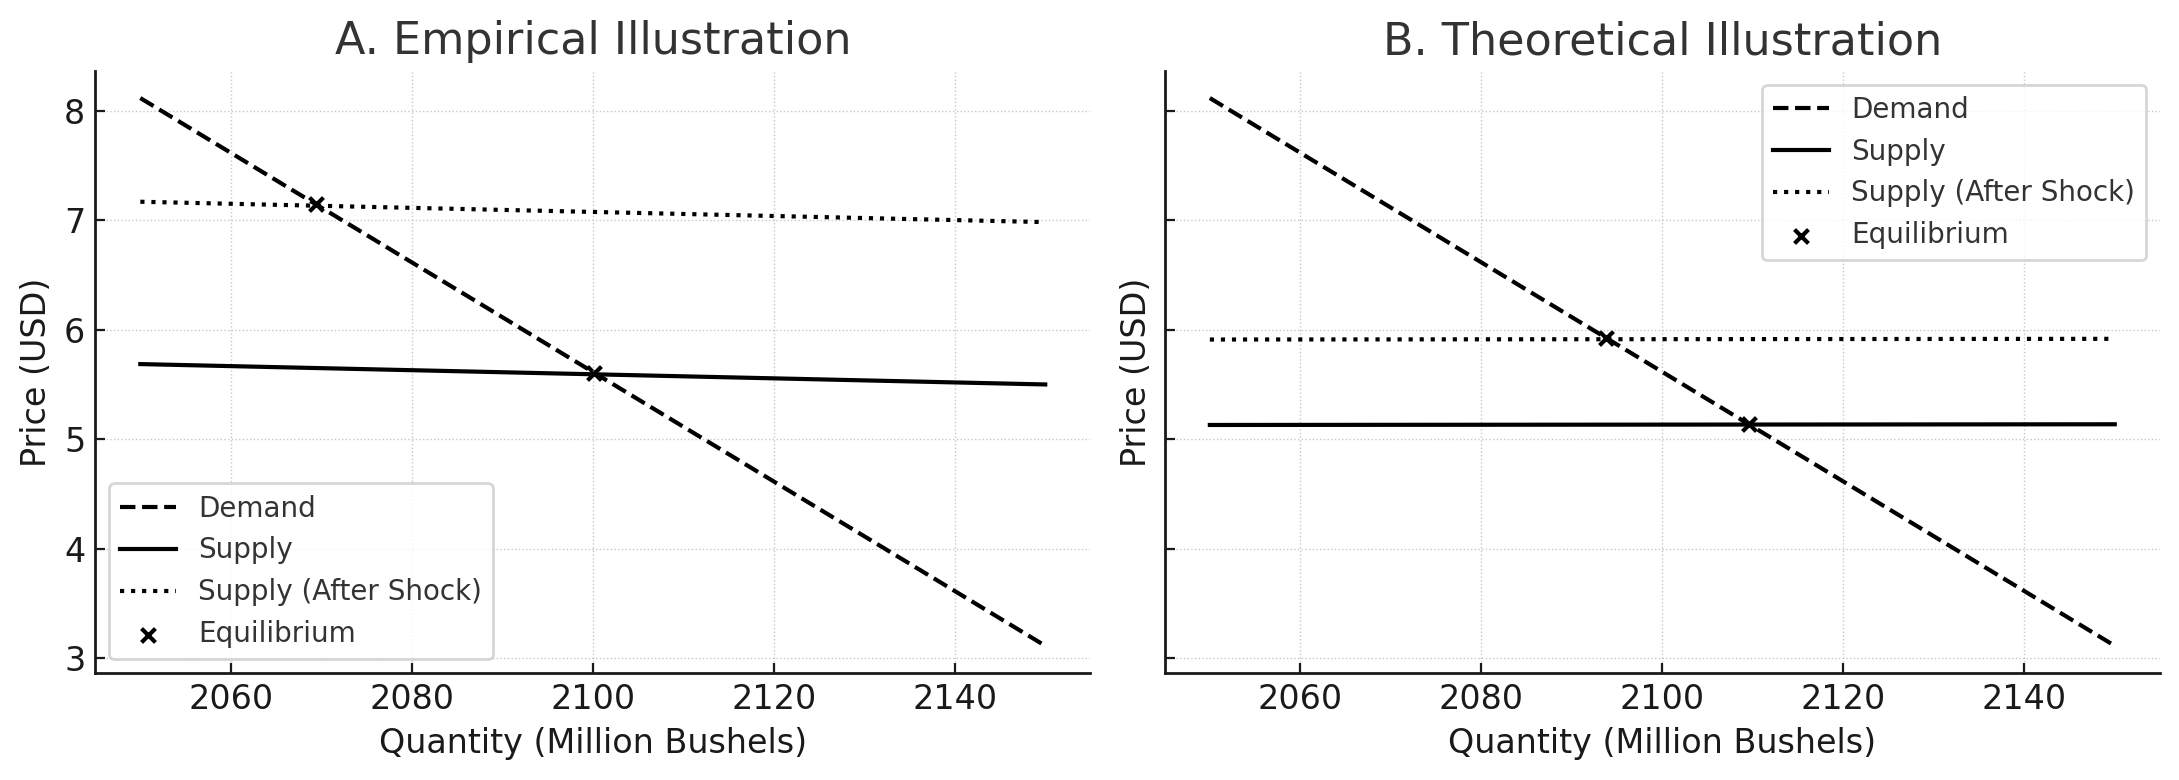
\includegraphics[width=\textwidth]{Hakenes illustration.png}
    \caption{\small{Comparison of empirical and theoretical supply responses to a 15.6\% shock in the U.S. wheat market. Panel A: Empirical supply estimated using OLS. Panel B: Theoretical supply based on the Hakenes–Schliephake (2024) model. Demand is held constant in both cases.}}
\end{figure}

\subsubsection{Structural Sources of Difference in Emissions Outcomes}

Although the same demand curve was used in both the empirical and theoretical approaches, the estimated reduction in carbon footprint differed considerably. The empirical estimation yielded a reduction of 359.36 million kg CO\textsubscript{2}e, while the theoretical model predicted a more modest reduction of 175.06 million kg CO\textsubscript{2}e.

This difference can be attributed entirely to the way supply was modeled. In the empirical estimation, the supply curve was estimated via OLS using observed data on price and quantity. This approach captured market behavior as it appeared in the historical record but did not account for underlying decision-making under uncertainty or equilibrium responses. In contrast, the theoretical supply curve was derived from the model’s structural assumptions, incorporating risk preferences, investment volatility, and optimal capital allocation. It reflected how households would respond to market changes under forward-looking behavior, leading to a more muted response in output and, correspondingly, in emissions.

Additionally, the theoretical model introduced a consequentialist perspective by assigning carbon responsibility based on the marginal impact of a household's consumption or investment. In doing so, it internalized substitution effects and capital reallocation, which were not accounted for in the empirical estimation. As a result, while the same emissions formula was applied in both cases, the theoretical model predicted a smaller footprint change due to the buffering effects of equilibrium adjustments. This difference underscores the importance of integrating behavioral dynamics into footprint assessment, particularly when evaluating the impact of shocks or policy interventions.


\section{Responsibility for Household Carbon Emissions}

Households are often portrayed as central actors in climate mitigation—urged to fly less, retrofit their homes, shift their diets, or reduce electricity use. Yet, the basis on which such responsibility is assigned remains contested. What does it mean to hold a household responsible for climate change, and how do we ensure that this responsibility is fair, actionable, and grounded in reality?

Existing carbon accounting methods offer different answers. Some emphasize direct control over emissions, others focus on consumption or supply chains, and still others ask whether a household’s actions actually reduce emissions. These differences reflect deeper questions about agency, influence, and obligation. 

This chapter rethinks household responsibility by comparing the attribution logics embedded in four key models—production-based (GHG Protocol), product-based (LCA), demand-based (EEIO), and marginal impact models (Hakenes and Schliephake). The aim is to evaluate not only how these methods measure emissions, but also how they construct the idea of responsibility itself and with what consequences for policy, fairness, and climate action.

\subsection{Attribution Principles}

\subsubsection{Attribution Based on Operational Control}

Control-based attribution allocates emissions to the actor who directly controls the physical source of greenhouse gas release. Emissions are assigned based on \textit{operational responsibility}, that is, who manages the combustion process or industrial activity rather than on who benefits from or demands the resulting goods and services. In this framework, emissions from electricity generation are attributed to power plants, and those from food or goods production are attributed to manufacturing firms, not to the households that consume the outputs.

The GHG Protocol is the principal framework that operationalizes this logic. In household-level applications, it typically attributes emissions only from direct fuel use (e.g., home heating, personal vehicles) and from purchased electricity or heat (Scopes 1 and 2). Emissions embedded in goods, services, or infrastructure (commonly classified as Scope 3) are excluded unless separately modeled. As a result, household responsibility appears significantly lower than in consumption-based frameworks. For instance, while households in developed economies are responsible for an estimated 60–70\% of emissions under a consumption-based approach, control-based inventories typically attribute only 10–20\% to them.\footnote{See Hertwich and Peters (2009). Consumption-based GHG emissions. \textit{Environmental Science \& Technology}.}

This method reflects a production-based understanding of responsibility: households are held accountable for emissions they physically generate or for energy they purchase, but not for upstream emissions embodied in their consumption. Although narrower in scope, this attribution style serves a clear regulatory function. Its operational clarity makes it particularly suitable for emissions inventories, carbon pricing schemes, and supply-side decarbonization policies that target industrial emitters rather than individuals. The GHG Protocol underpins most national reporting systems and corporate disclosures, and is explicitly aligned with policy instruments such as emissions caps, sectoral mitigation targets, and producer-level carbon accounting.\footnote{See World Resources Institute and WBCSD (2004). \textit{The Greenhouse Gas Protocol: A Corporate Accounting and Reporting Standard}. Also see den Elzen et al. (2020), \textit{Nature Climate Change}, on policy alignment of production-based accounting.} By tracing emissions to producers rather than consumers, control-based attribution enables system-level mitigation efforts without requiring detailed behavioral data at the household level.

\subsubsection{Consumption-Based Attribution}

Consumption-based attribution assigns responsibility for emissions to end users, based on the idea that consumer demand drives production and, ultimately, greenhouse gas emissions. Unlike control-based methods that assign emissions to producers, consumption-based frameworks trace emissions along the supply chain and allocate them to the final household that purchases or uses the good or service.

Among the methods reviewed in this paper, two approaches operationalize consumption-based attribution: life cycle assessment (LCA) and environmentally extended input–output (EEIO) models. Both assign emissions to households for the upstream impacts of their consumption, but they differ in analytical resolution and system boundaries. LCA focuses on product-level analysis by quantifying emissions over a product’s entire life cycle—from raw material extraction through use and disposal.\footnote{Curran, M. A. (2015). Life Cycle Assessment: Principles and Practice. EPA.} This method enables fine-grained comparisons of consumption choices (e.g., meat versus plant-based diets) and supports interventions like eco-labeling and sustainable procurement.

EEIO models, by contrast, estimate emissions based on monetary flows across sectors and are designed to capture systemic effects across entire economies. They link household expenditure data with environmental accounts using national input–output tables, assigning emissions in proportion to spending across categories such as food, transport, and housing.\footnote{Wiedmann, T. (2009). A review of recent multi-region input–output models used for consumption-based emission accounting. \textit{Ecological Economics}.} While LCA relies on detailed process-level data, EEIO models are structured around macroeconomic datasets, making them suitable for national-scale analysis and policy evaluation.

Both approaches consistently attribute a large share of global emissions to households, typically between 60\% and 70\% in high-income countries, by including indirect emissions embedded in consumption.\footnote{Ivanova, D. et al. (2016). Environmental impact assessment of household consumption. \textit{Journal of Industrial Ecology}.} This high attribution has made consumption-based methods influential in shaping narratives around individual climate responsibility and has informed the design of tools such as carbon footprint calculators, dietary guidelines, and voluntary offsetting schemes. However, these methods also risk overstating household agency by abstracting from structural constraints, supply-side inertia, and the availability of low-carbon alternatives.

Despite these limitations, consumption-based attribution provides valuable insights for policymaking. It highlights carbon-intensive lifestyle domains, supports the development of behavioral nudges and fiscal instruments (e.g., carbon taxes or subsidies), and enables differentiated climate strategies across income groups. In this way, it complements production-based models by identifying downstream leverage points for demand-side mitigation.

\subsubsection{Consequentialist Attribution}

The general equilibrium structure and derivation of the Hakenes and Schliephake (2024) model are presented in Chapter~7. Here, we focus specifically on how the model attributes responsibility for emissions—offering a fundamentally different logic from control- or consumption-based methods.

Consequentialist attribution links household responsibility to the actual change in total emissions resulting from marginal economic decisions. In contrast to attribution by operational control or average consumption, this approach estimates how much aggregate emissions would differ if a household were absent from the economy. The household’s carbon footprint is thus defined as the causal marginal impact of its consumption and investment choices on total emissions.

Within the Hakenes–Schliephake framework, emissions are attributed through a counterfactual comparison: the general equilibrium of the full economy versus the equilibrium that would occur if a given household did not participate. Because the model includes both product and financial markets, the resulting footprint incorporates not only direct effects but also indirect spillovers through price mechanisms, risk-adjusted investments, and inter-household substitution. The marginal impact of a household’s behavior is calculated using a weighting parameter, $\varphi$, which determines the relative attribution of emissions between consumption and investment.\footnote{Hakenes, H. \& Schliephake, E. (2024). Your Carbon Footprint, Including Investments. SSRN 4710536. See also Section~7.1.4 in this thesis for derivation of $\varphi$.}

This weighting is sensitive to structural characteristics of the economy: greater risk aversion or financial volatility shifts responsibility toward consumption, while higher substitutability across sectors amplifies the spillover effect through investment. As a result, households are only held responsible for emissions they can meaningfully influence. If consumption is perfectly substitutable or investment flows are fully absorbed by other agents, the attributed footprint may approach zero—even if the household’s nominal expenditure is large.

By assigning responsibility based on marginal system-wide impact, the model avoids double-counting and mitigates the over-attribution seen in static frameworks. It also aligns well with policy approaches that emphasize structural levers, such as green financial regulation or carbon-intensity weighting of investment portfolios. While less intuitive and more data-intensive than other methods, this attribution logic provides a refined lens for distinguishing symbolic from substantive household climate action.

\subsection{Comparative Synthesis of Attribution Frameworks}

Attribution methods differ not only in analytical structure but in how they frame responsibility—what they assign to households, what they assume about agency, and what they ignore. As visualized in Figure~\ref{fig:heatmap}, these differences create meaningful trade-offs that shape both interpretation and policy relevance.

Control-based attribution (GHG Protocol) limits household responsibility to direct actions, minimizing the risk of over-attribution but offering little behavioral or structural insight. Consumption-based approaches (LCA and EEIO) invert this: they assign large shares of emissions to households, enabling lifestyle-oriented analysis but often abstracting from real-world constraints, rebound effects, or structural inertia. They perform well descriptively but struggle to differentiate between symbolic and effective action.

Only the Hakenes and Schliephake model formally incorporates systemic feedbacks. Its consequentialist logic reframes attribution as marginal influence, not average burden. This avoids double-counting and grounds responsibility in causal agency, but at the cost of complexity, abstraction, and limited communicability.

Figure~\ref{fig:heatmap} illustrates this spectrum: methods differ in how much they reveal about behavioral influence, how they treat economic structure, and how carefully they delimit the scope of household responsibility. Choosing an attribution framework is therefore not just a technical exercise—it reflects underlying assumptions about fairness, tractability, and what forms of action are worth encouraging.

\begin{figure}[h]
    \centering
    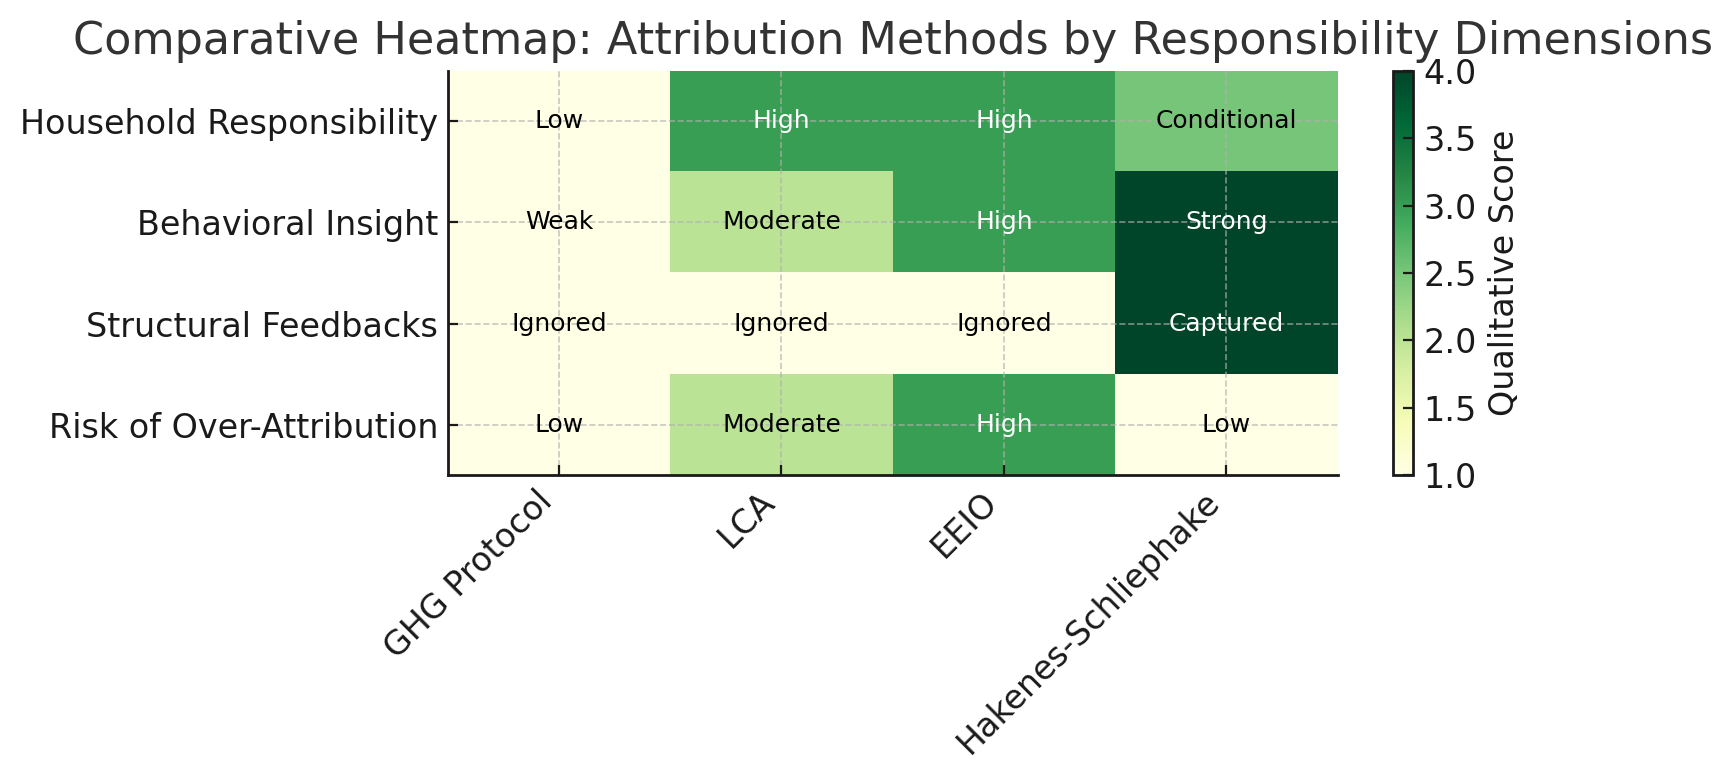
\includegraphics[width=\textwidth]{attribution_heatmap.png}
    \caption{Comparative heatmap of attribution frameworks across key responsibility dimensions. Higher scores indicate greater behavioral relevance, structural sensitivity, or risk of over-attribution. Source: Author's own analysis based on Hertwich and Peters (2009), Ivanova et al. (2016), Hakenes and Schliephake (2024), and Capstick et al. (2019).}
    \label{fig:heatmap}
\end{figure}

\noindent
This synthesis sets the stage for the next chapter, where we assess how different attribution logics align with climate policy instruments and what this implies for equitable mitigation strategies.

\section{Comparative Reflections on Policy Instruments for Household Decarbonization}

Climate mitigation efforts increasingly recognize households as both contributors to and potential levers for reducing global greenhouse gas (GHG) emissions. Yet the policy instruments aimed at curbing household carbon footprints vary substantially in design, scope, and effectiveness—a variation largely shaped by the underlying method used to calculate those emissions. Whether a policy is targeted at fuel use, investment decisions, dietary choices, or broader patterns of consumption depends on whether emissions are accounted for through direct measurement (as in the GHG Protocol), product life cycles (LCA), system-wide economic flows (EEIO), or general equilibrium models that incorporate behavioral and financial spillovers (e.g., Hakenes and Schliephake).

Each of these methods carries implicit assumptions about responsibility, agency, and feasibility. As a result, the policies they inform often differ not only in their technical design but also in their capacity to deliver equitable and durable decarbonization. While LCA-informed policies tend to focus on greening products, EEIO approaches shift attention to consumption patterns and supply chains, and income-based models emphasize structural inequalities in both emissions and responsibility. Yet these models often fail to incorporate the complex social and behavioral drivers of energy use at the household level, particularly in developing contexts where informality, aspiration, and cultural norms play a decisive role. Additionally, emerging technologies such as artificial intelligence (AI) offer new avenues for real-time monitoring and behavioral nudging but must be deployed thoughtfully to avoid reinforcing inequities.

This chapter analyzes policy instruments for household decarbonization through a methodological lens, examining how different models shape policy design and impact. It integrates recent insights from behavioral science, climate finance, and digital governance to evaluate not only which policies work, but \emph{why}, \emph{where}, and \emph{for whom} they are most effective.

The effectiveness and fairness of policies aimed at reducing household carbon footprints depend not only on the political and institutional context in which they are implemented, but also on the method used to estimate emissions. This section classifies key climate policy instruments relevant to households—such as carbon taxes, cap-and-trade schemes, product standards, investment-based levies, and behavioral interventions—and evaluates their suitability through the lens of different carbon accounting methods: the GHG Protocol, Life Cycle Assessment (LCA), Environmentally Extended Input-Output (EEIO) analysis, and the general equilibrium model by Hakenes and Schliephake.

Rather than examining the models first, this section reverses the typical approach and begins with the policies themselves. For each instrument, we consider which methodological framework provides the strongest analytical basis and what implications arise for policy design and equity.

\subsection{Carbon Taxes}

Carbon taxation is one of the most widely implemented and theoretically robust instruments for climate mitigation. Designed to internalize the social cost of carbon, it levies a uniform price on each tonne of CO\textsubscript{2} equivalent emissions, thereby incentivizing behavioral change and technological substitution across sectors. In the context of households, carbon taxes primarily influence consumption through higher prices for fossil fuels, electricity, heating, and carbon-intensive goods. 

The implementation of carbon taxes varies considerably across national contexts. Scandinavian countries such as Sweden and Finland have adopted high carbon tax rates targeting transport and heating fuels, achieving measurable reductions in per capita emissions. In contrast, countries like Chile and South Africa have introduced modest levies with narrower sectoral coverage. These taxes are typically passed down to consumers, making them salient at the household level. However, their effectiveness and fairness hinge on critical design parameters, including the tax rate, the breadth of emissions covered, and the extent to which revenues are redistributed to mitigate regressive effects.

From a methodological standpoint, carbon taxes have historically been grounded in the accounting principles of the Greenhouse Gas (GHG) Protocol. This framework, which emphasizes direct (Scope 1) and energy-related (Scope 2) emissions, provides a transparent and standardized basis for taxing household fossil fuel use. Nevertheless, its reliance on territorial emissions accounting has significant limitations, particularly in high-income countries where a substantial share of emissions is embodied in imported goods and services. Policies based solely on this protocol risk underestimating household responsibility and misallocating incentives.

A more comprehensive foundation is offered by Environmentally Extended Input-Output (EEIO) models, which capture the full lifecycle emissions associated with household consumption. EEIO-based approaches enable the design of consumption-based carbon taxes that target emissions embedded in goods—such as food, electronics, or clothing—regardless of their country of origin. These models thus support the development of more equitable and globally consistent taxation schemes, including border carbon adjustments and differentiated VAT structures. Moreover, they allow policymakers to trace emissions along complex supply chains, aligning fiscal instruments with actual carbon accountability.

While carbon taxes are generally lauded for their simplicity, cost-effectiveness, and technological neutrality, they are not without drawbacks. Empirical evidence suggests that low-income households tend to spend a larger share of their income on energy and food, raising concerns about regressivity. Without targeted compensation or revenue recycling mechanisms, carbon taxes risk exacerbating social inequality. Conversely, taxes informed by EEIO analysis offer the possibility of aligning environmental effectiveness with distributive justice by incorporating upstream emissions and differentiating taxation by product class or expenditure profile.

Ultimately, the policy effectiveness of carbon taxation depends on aligning its design with an accurate and comprehensive understanding of household emissions. Models limited to direct emissions can inform short-term pricing measures but fail to capture structural drivers. In contrast, EEIO models—though more data-intensive—support systemic interventions that better reflect the embeddedness and inequality of household carbon footprints.

\subsection{Product and Appliance Standards}

Product and appliance standards constitute one of the most mature and widely adopted policy instruments for reducing household carbon emissions. These standards typically target energy consumption at the point of use—such as lighting, refrigeration, heating, and cooking—and have been implemented in forms ranging from mandatory minimum energy performance standards (MEPS) to voluntary eco-labels and public procurement guidelines. By setting thresholds for efficiency or lifecycle emissions, such policies aim to reduce the environmental intensity of routine household consumption without requiring active behavioral change.

The methodological basis for product standards lies primarily in Life Cycle Assessment (LCA), which enables regulators to assess cradle-to-grave emissions associated with household goods. In contrast to direct emissions accounting under the GHG Protocol, LCA captures the embedded carbon in both the production and end-use phases, making it particularly suitable for targeting emissions-intensive consumption categories such as food systems, home appliances, and construction materials. This approach is visible in the European Union’s Ecodesign Directive and the widespread adoption of appliance labeling schemes across OECD countries. Japan’s Top Runner Program extends this logic by continuously updating energy efficiency baselines based on the best-performing technologies available in the market.

However, the success of such standards depends not only on technical design but also on affordability, cultural fit, and enforcement capacity. Greenwood and Warren (2022) emphasize that the deployment of energy-efficient appliances—such as clean cookstoves or refrigerators—is often embedded in complex behavioral and aspirational landscapes. For instance, in low-income contexts, product choice is rarely governed by lifecycle performance metrics alone; it is also shaped by symbolic preferences, perceived modernity, and gendered divisions of domestic labor. This disconnect can lead to underutilization of subsidized technologies or parallel use alongside traditional devices—a phenomenon known as “fuel stacking.”

Climate finance mechanisms have increasingly supported product and appliance standards, particularly through results-based financing and concessional lending. Programs such as the Green Climate Fund and bilateral initiatives have funded appliance swaps, low-carbon public housing, and rural electrification projects aimed at modernizing household technology. Yet, without integrated behavioral design or inclusive co-creation, such interventions often underperform in both uptake and sustained emissions reduction.

Moreover, LCA-based standards tend to privilege measurable product categories over complex service chains or informal markets. While these tools excel at regulating formal-sector appliances, they are less effective at addressing emissions associated with informal food processing, construction, or transportation services common in the Global South. In such settings, simplified hybrid models or community-led appliance design may offer more context-sensitive alternatives.

Ultimately, product and appliance standards reflect a technocratic vision of household decarbonization—one in which emissions reductions are achieved through the restructuring of markets and the imposition of universal thresholds. While such instruments have contributed significantly to mitigation in high-income countries, their broader effectiveness depends on coupling lifecycle logic with affordability, symbolic relevance, and climate finance that enables widespread access.

\subsection{Investment-Based Instruments}

While household carbon policies have traditionally focused on consumption patterns, a growing body of research suggests that investment decisions—particularly among high-income households—play an equally, if not more, significant role in driving emissions. Investment-based instruments seek to address this blind spot by attributing emissions responsibility to financial flows, capital holdings, and shareholder influence over high-emitting sectors. These policies include carbon-adjusted income taxation, green investment mandates, and climate-aligned fiduciary standards for institutional investors.

The methodological foundation for such instruments departs significantly from territorial or product-based accounting frameworks. Instead, it aligns more closely with general equilibrium approaches such as the model proposed by Hakenes and Schliephake, which internalize spillovers, substitutability, and risk allocation across sectors. By modeling households not just as consumers but also as portfolio holders, these frameworks reveal a more comprehensive carbon responsibility landscape—one that links emissions to risk-bearing decisions and capital endowments. Under such a view, carbon pricing should not only apply at the point of fuel use or product purchase, but also at the point of investment in emissions-intensive industries.

Empirical support for this approach is found in the work of Starr et al. (2023), who demonstrate that in the United States, the top 10\% of households are responsible for over 40\% of emissions, largely through investment-related income. The top 1\% alone account for nearly 17\% of national emissions, despite far lower shares in direct consumption. These findings challenge the prevailing focus on lifestyle nudges and energy efficiency campaigns, suggesting instead that capital taxation, green bond regulation, and shareholder accountability mechanisms may be more effective levers for structural decarbonization.

Policy instruments emerging from this insight are diverse. One proposal is an income-based carbon tax that includes capital gains, dividends, and rents, weighted by the carbon intensity of the underlying assets. Another is the integration of climate risk into fiduciary duty, thereby requiring institutional investors to divest from high-emitting sectors or face legal exposure. Public finance mechanisms such as sovereign wealth funds or central bank green mandates can also be oriented to reward low-carbon investment behavior. While these approaches are still politically nascent, their analytical foundation is increasingly robust.

Climate finance can play a catalytic role in operationalizing these instruments. By de-risking green investments or supporting blended finance structures, multilateral funds can influence private capital allocation at scale. However, doing so requires a departure from conventional project-based finance logic toward systems-oriented intervention. It also necessitates governance reforms in how emissions responsibility is assigned across the financial system.

Unlike traditional instruments that focus on changing household behavior through prices or nudges, investment-based approaches confront the structural reproduction of carbon intensity through asset ownership and financial intermediation. They offer a more ambitious, albeit politically challenging, framework for carbon responsibility—one that implicates privilege, long-term risk, and the ethics of capital deployment.

\subsection{Behavioural Interventions}

Behavioural interventions target the social, psychological, and cultural drivers of household carbon emissions, offering a critical complement to price-based and technological policies. These instruments aim to shift preferences, norms, and routines—such as cooking habits, appliance use, or mobility patterns—through strategies like public education campaigns, symbolic media, community co-design, and default-setting. Their rationale lies in the recognition that household behavior is not merely a function of economic incentives or technological availability, but deeply embedded in identity, aspiration, and social context.

Climate finance has increasingly supported such interventions, particularly in the Global South, where formal energy infrastructure is often limited and behavior constitutes a primary leverage point for emissions reduction. Yet, as Greenwood and Warren (2022) argue, many of these efforts fail to achieve durable impact because they rely on top-down diffusion models that misunderstand or overlook local complexity. For instance, clean cookstove distribution programs, despite substantial investment, have often been met with low adoption rates or rapid abandonment—not due to lack of access, but because the new technologies failed to align with culinary practices, gender roles, or symbolic values associated with modernity and tradition.

More successful examples emphasize co-creation and narrative reframing. Kenya’s “Samba Chef” program, which used reality television to model aspirational clean cooking behaviors, is one such case. By embedding energy transitions into culturally resonant storylines, it shifted attitudes in ways that technical interventions could not. Similar results have been found in participatory appliance design projects in Zambia and India, where involving users—particularly women—in the specification and aesthetics of new technologies led to significantly higher uptake and consistent use.

Methodologically, behavioural interventions are often under-theorized within carbon accounting models. Conventional frameworks such as the GHG Protocol or LCA assume stable preferences and linear use patterns, rendering them ill-suited to capture the fluidity of household behavior. Even EEIO models, while broader in scope, typically aggregate behavioral heterogeneity into average sectoral flows. As a result, many high-resolution opportunities for targeted intervention remain invisible to these approaches.

The emerging intersection of behavioural science and climate finance seeks to address this gap by funding programs that test nudges, defaults, and social proof interventions through randomized trials and adaptive evaluation. However, scaling these efforts requires new metrics for impact that go beyond kilowatt-hours saved or emissions averted. Metrics must account for persistence, spillover, and equity—particularly when interventions disproportionately affect women, informal workers, or culturally marginalized groups.

Ultimately, behavioural interventions are indispensable for household decarbonization not because they replace structural reform, but because they determine whether such reforms are accepted, adapted, and sustained. When supported by climate finance that is responsive to context, aspiration, and voice, these interventions can unlock forms of mitigation that are both low-cost and high-trust. Without them, even the most sophisticated technologies risk remaining unused, and the most ambitious policies risk becoming irrelevant.

\subsection{AI and Digital Tools}

Artificial intelligence (AI) and digital tools are emerging as pivotal instruments for enhancing the precision, personalization, and policy relevance of household carbon footprint mitigation. These technologies enable real-time data collection, personalized feedback, and dynamic emissions modelling—functions that are largely beyond the reach of conventional policy instruments. When deployed responsibly, AI-based systems can help close the feedback loop between consumption decisions and environmental impact, especially for urban and digitally connected households.
The primary methodological advantage of AI lies in its ability to integrate high-dimensional, heterogeneous data across behavioral, financial, and environmental domains. For instance, machine learning models can estimate household emissions by combining transaction-level expenditure data, geospatial information, energy usage patterns, and demographic profiles. These approaches enhance the granularity of footprint estimation beyond the sectoral averages found in Environmentally Extended Input-Output (EEIO) models, and offer dynamic adaptability to behavioral change—a limitation of traditional Life Cycle Assessment (LCA) frameworks. A recent study on the evolution of household carbon research highlights how contextual language models and unsupervised clustering can extract nuanced trends and policy gaps from large bibliometric datasets, offering new tools for targeting emissions hotspots and informing targeted interventions.


In practical terms, AI is being embedded into mobile applications, smart meters, and digital nudging platforms. For example, apps such as Svalna and Klima allow users to track their carbon emissions in real-time, simulate alternative consumption scenarios, and receive behavioral recommendations. Other tools use AI to automate carbon accounting for household investment portfolios, aligning with investment-based attribution models. The convergence of AI with fintech platforms is also enabling embedded carbon pricing in personal budgeting tools, which could support low-carbon transitions at scale if governed transparently.

Climate finance institutions are beginning to recognize the role of digital tools in accelerating household decarbonization. Digital public infrastructure investments—such as open emissions APIs, energy data hubs, and secure identity-linked carbon registries—are being supported through development finance initiatives. However, as Greenwood and Warren (2022) caution, such innovations risk reproducing existing inequalities if not designed with digital access, literacy, and data privacy at the core. In low-income and rural settings, where smartphone penetration and broadband access remain limited, reliance on AI may exacerbate marginalization rather than empower mitigation.

Moreover, algorithmic opacity and commercial ownership of data raise concerns about accountability and consent in emissions tracking. Without robust governance frameworks, digital tools may incentivize superficial compliance over substantive change. There is also a risk of reinforcing individual responsibility narratives while deflecting attention from structural emissions drivers—a critique increasingly directed at platform-based sustainability solutions.

Nonetheless, when deployed in alignment with participatory design, open standards, and context-sensitive financing, AI and digital tools can significantly enhance the reach and responsiveness of household carbon policies. By enabling adaptive, real-time feedback and unlocking granular emissions data, they create new pathways for climate finance to engage households not merely as emitters, but as co-designers of a low-carbon future.

\subsection{Integrating Instruments and Equity}

The five policy instruments examined in this chapter—carbon tax, product standards, investment-based taxation, behavioural interventions, and AI-enabled digital tools—each emerge from different methodological traditions and assign carbon responsibility in distinct ways. What unites them, however, is their relevance to the household as both emitter and agent. By pairing these instruments with the methods that best support their design—whether LCA, EEIO, general equilibrium modeling, or behavioural science—we gain clarity not only about which tools are technically appropriate, but also about which are ethically justified, socially acceptable, and financially scalable. The table below summarizes this alignment and reflects on the broader implications for climate policy and finance at the household level.


\begin{table}[h]
\centering
\caption{Household Carbon Policy Instruments: Methodological Alignment and Strategic Implications}
\label{tab:final_policy_comparison}
\begin{threeparttable}
\resizebox{\textwidth}{!}{%
\begin{tabular}{L{3.8cm} L{4.2cm} L{3.3cm} L{3.8cm} L{4cm}}
\toprule
\textbf{Policy Instrument} & \textbf{Methodological Basis} & \textbf{Climate Finance Compatibility} & \textbf{Strengths} & \textbf{Limitations} \\
\midrule
Carbon Taxes & GHG Protocol (Scope 1–2); extended by EEIO for consumption-based pricing & Moderate\tnote{1} & Transparent, administratively simple; scalable across sectors & Regressive without redistribution; ineffective without embedded emissions accounting \\
\addlinespace
Product and Appliance Standards & Life Cycle Assessment (LCA); partially supported by GHG Protocol & High\tnote{2} & Technologically mature; harmonized with global trade and procurement policies & Poor alignment with cultural practice; limited uptake in informal settings \\
\addlinespace
Investment-Based Instruments & General Equilibrium (Hakenes-Schliephake), supported by EEIO & Moderate\tnote{3} & Targets systemic inequality and capital-linked emissions; long-term structural potential & Requires fiscal system reform; politically sensitive in high-income contexts \\
\addlinespace
Behavioural Interventions & Behavioural science; weakly embedded in traditional carbon models & High\tnote{4} & Low-cost, participatory, socially adaptive; crucial in informal or transitional settings & Difficult to quantify and fund through conventional carbon metrics; often undervalued \\
\addlinespace
AI and Digital Tools & Hybrid: EEIO + LCA + behavioural integration & Growing\tnote{5} & Enables real-time, household-specific carbon tracking; bridges data with policy simulation & Digital exclusion risks; regulatory and privacy concerns in implementation \\
\bottomrule
\end{tabular}
}
\vspace{1em}
\begin{tablenotes}
\footnotesize
\item[1] Adopted in Sweden, Canada, and Chile; climate finance relevance via carbon dividends and fiscal transition funding.
\item[2] Supported by GCF, bilateral donors, and national public procurement standards (e.g., EU Ecodesign Directive).
\item[3] Potential integration into sovereign wealth funds, IMF tax proposals, and fiduciary regulation.
\item[4] Increasingly funded via GEF and UNDP behavioral pilots, especially where co-benefits (e.g., health, gender) apply.
\item[5] Enabled through blended finance, fintech partnerships, and smart city infrastructure initiatives.
\end{tablenotes}
\end{threeparttable}
\end{table}

This comparative analysis highlights that no single methodological framework or policy instrument is sufficient to address the complexity of household carbon emissions. While the GHG Protocol and LCA provide standardized tools for measuring and regulating direct and product-specific emissions, they risk oversimplifying the social, financial, and behavioral structures that underpin household carbon responsibility. EEIO and general equilibrium models offer more comprehensive representations of systemic responsibility—particularly in the context of investment and inequality—but require data-intensive infrastructure and institutional coordination. Similarly, behavioural interventions and AI-enabled tools introduce much-needed responsiveness and granularity, yet remain underutilized in formal climate finance pipelines and carbon accounting systems.

The instruments most likely to succeed are those designed with both methodological precision and social fit. Effective household decarbonization will not result from technical superiority alone, but from the integration of upstream and downstream logics: investment-linked responsibility, consumption-based accountability, behavioral relevance, and real-time feedback. Climate finance must evolve to reflect this layered reality—shifting from discrete funding streams to portfolios that embed digital, behavioral, and structural insights within a unified mitigation strategy. The next chapter takes this synthesis forward, identifying key design principles and policy pathways for constructing such an integrated approach.

\subsection{Policy Implications and Strategic Recommendations}

The comparative analysis presented in this chapter underscores that effective household decarbonization cannot be achieved through technical instruments alone. Each methodological approach—whether focused on direct emissions, product life cycles, system-wide consumption, or capital flows—reveals distinct layers of responsibility and intervention. Therefore, policy design must be layered accordingly: tailored to method, responsive to social context, and structurally aligned with available climate finance mechanisms.

For national governments, the implication is twofold. First, carbon taxes and appliance standards must be informed by consumption-wide accounting frameworks such as EEIO, not just territorial emissions. This allows for the inclusion of imported emissions and avoids unjustly penalizing lower-income households while exempting capital-intensive lifestyles. Second, policy instruments must be evaluated not only on their mitigation potential but also on their distributional consequences. Incorporating income-linked carbon pricing or capital-based taxation—as proposed in equilibrium models—offers a pathway to align climate goals with fiscal justice.

Climate finance institutions must evolve beyond a narrow project-based logic to support integrated portfolios that combine digital, behavioral, and structural interventions. This means financing not only solar panels and cookstoves, but also carbon tracking apps, participatory media, and public goods infrastructure that enhances agency. Behavioural interventions, in particular, should be elevated from peripheral pilots to core strategy, especially in adaptation and just transition frameworks.

City-level policymakers and infrastructure agencies should adopt hybrid carbon accounting methods that combine EEIO data with behavioural and spatial analytics. Urban households are not only dense emitters but also highly sensitive to transport design, food access, and housing policy. AI-enabled monitoring tools can help local governments visualize real-time emissions and target interventions more precisely—but only if they are designed for inclusivity and digital equity.

Finally, academic and statistical communities have a critical role in reshaping how emissions responsibility is measured. Methodological choices are not neutral: they shape which policies are seen as legitimate and which lives are made visible in carbon governance. Standard-setting bodies and data providers should work toward frameworks that reflect both structural causes and behavioural textures of emissions. This includes expanding household surveys to capture investment flows, informal energy use, and digital access.

In sum, effective household carbon policy must be methodologically informed, equity-sensitive, and operationally realistic. The next chapter concludes by reflecting on how integrating these elements redefines the boundary between personal responsibility and structural transformation in climate action.

\section{Conclusion}

This thesis set out to examine how the method used to calculate household carbon footprints shapes the policies that follow, the responsibilities that are assigned, and the equity outcomes that result. By comparing four dominant frameworks—the GHG Protocol, Life Cycle Assessment (LCA), Environmentally Extended Input-Output (EEIO) models, and the general equilibrium model by Hakenes and Schliephake—this study has shown that carbon accounting is not merely a technical exercise, but a deeply political one. The choice of method influences not only the scale and location of emissions, but also the narrative of blame and the distribution of accountability.

Empirical illustrations revealed that the estimated footprint of a household can vary dramatically depending on whether emissions are measured directly, traced through product life cycles, allocated via supply chains, or adjusted for investment-driven influence. These differences are not just numerical—they are normative. They determine who is asked to change, who is allowed to continue, and whose behavior is rendered visible or invisible in policy discourse.

The analysis of policy instruments further demonstrated that certain methods lend themselves to particular forms of intervention. Carbon taxes and appliance standards are most coherent under GHG and LCA frameworks, while EEIO models support structural taxation and global trade instruments. Investment-based responsibility, supported by equilibrium modelling, remains underexplored but is crucial for targeting the disproportionate carbon influence of the wealthiest households. Behavioural and digital tools cut across these methods, providing adaptability and granularity where structural models fall short.

A key contribution of this thesis lies in showing that household carbon responsibility is layered—simultaneously behavioral, infrastructural, and financial. Effective climate policy must therefore be layered as well: combining short-term nudges with long-term structural reforms, and integrating traditional emissions models with behavioral science and real-time digital infrastructure. Climate finance, too, must evolve to support this complexity—not just by funding technologies, but by enabling fairness, participation, and visibility.

The limitations of this study—most notably the simplified empirical illustrations and the use of stylized rather than field-based data—suggest several avenues for future research. These include applying the Hakenes-Schliephake model to real-world portfolio data, testing AI-powered carbon trackers in diverse urban contexts, and evaluating how responsibility shifts under hybrid or evolving accounting methods.

At a moment when climate responsibility is increasingly individualized in public discourse, this thesis argues for a more systemic and just understanding of household emissions. It is not only what we consume, but how we are positioned—economically, socially, and institutionally—that defines our footprint. By interrogating the methods beneath the metrics, we may arrive at policies that are not only effective, but fair.

\newpage

\appendix
\section*{Appendix A: Tables and Figures}

\renewcommand{\thetable}{A\arabic{table}}
\renewcommand{\thefigure}{A\arabic{figure}}
\setcounter{table}{0}
\setcounter{figure}{0}


\begin{table}[H]
\captionsetup{justification=raggedright,singlelinecheck=false} 
\caption{Annual number of publications, cumulative total, and estimated annual growth rate in household carbon footprint literature (2000–2025).}
\resizebox{0.8\textwidth}{!}{%
\begin{tabular}{rrrr}
\toprule
Year & Number of Publications & Cumulative Publications & Annual Growth (\%) \\
\midrule
2006 & 2 & 2 & 0.00 \\
2007 & 3 & 5 & 50.00 \\
2008 & 5 & 10 & 66.67 \\
2009 & 13 & 23 & 160.00 \\
2010 & 17 & 40 & 30.77 \\
2011 & 31 & 71 & 82.35 \\
2012 & 30 & 101 & -3.23 \\
2013 & 39 & 140 & 30.00 \\
2014 & 45 & 185 & 15.38 \\
2015 & 59 & 244 & 31.11 \\
2016 & 57 & 301 & -3.39 \\
2017 & 76 & 377 & 33.33 \\
2018 & 86 & 463 & 13.16 \\
2019 & 92 & 555 & 6.98 \\
2020 & 115 & 670 & 25.00 \\
2021 & 142 & 812 & 23.48 \\
2022 & 110 & 922 & -22.54 \\
2023 & 134 & 1056 & 21.82 \\
2024 & 171 & 1227 & 27.61 \\
2025 & 84 & 1311 & - \\
\bottomrule
\end{tabular}
}
\raggedright
\vspace{0.3cm}

\footnotesize Source: Scopus. (n.d.). Search for "household carbon footprint" using the advanced search. July 2025, from [https://www.scopus.com]
\end{table}

\begin{table}[H]
\captionsetup{justification=raggedright,singlelinecheck=false} 
\caption{Top 10 contributing authors in HCF literature and their affiliations.}
\resizebox{\textwidth}{!}{%
\begin{tabular}{llr}
\toprule
Author & Affiliation & Publications \\
\midrule
Long Y. &  The University of Tokyo, Tokyo, Japan & 24 \\
Li J. & School of Economics, Beijing Institute of Technology, China & 19 \\
Shigetomi Y. & Graduate School of Environmental Studies, Tohoku University, Japan & 18 \\
Wang Y. & School of Finance, Yunnan University of Finance and Economics, China & 17 \\
Heinonen J. & Faculty of Civil and Environmental Engineering, Tampere University, Finland & 17 \\
Zhang Y. & School of Economics and Management, Tianjin Agricultural University, China & 15 \\
Yoshida Y. & School of the Environment, Nanjing University, China & 15 \\
Li Y. & SJTU-UNIDO Joint Institute of Inclusive and Sustainable Industrial Development, China & 15 \\
Wang J. & College of Resources and Environmental Sciences, China Agricultural University & 14 \\
Hubacek K. & Institute of Carbon Neutrality, Peking University, China & 14 \\
\bottomrule
\end{tabular}
}
\raggedright
\vspace{0.3cm}

\footnotesize Source: Author's own analysis from Scopus. (n.d.) dataset. Search for "household carbon footprint" using the advanced search. July 2025, from [https://www.scopus.com]

\end{table}

\begin{table}[H]
\captionsetup{justification=raggedright,singlelinecheck=false} 
\caption{Top 10 most frequently used keywords in HCF literature.}
\resizebox{0.4\textwidth}{!}{%
\begin{tabular}{lr}
\toprule
Keyword & Frequency \\
\midrule
carbon footprint & 305 \\
climate change & 91 \\
life cycle assessment & 67 \\
household consumption & 59 \\
greenhouse gas emissions & 56 \\
sustainability & 41 \\
food waste & 37 \\
input-output analysis & 37 \\
household & 35 \\
carbon emissions & 34 \\
\bottomrule
\end{tabular}
}
\raggedright
\vspace{0.3cm}

\footnotesize Source: Author's own analysis from Scopus. (n.d.) dataset. Search for "household carbon footprint" using the advanced search. July 2025, from [https://www.scopus.com]
\end{table}

\begin{table}[H]
\centering
\caption{Mean Consumption Expenditure per Household, Structure (\%), Annual Rate (\%) and
 Absolute Difference by ECOICOP divisions. Year 2022}\label{tab:expenditure}
\resizebox{\textwidth}{!}{
\begin{tabular}{l S[table-format=5.0] S[table-format=5.1] S[table-format=2.1] S[table-format=5.0]}
\toprule
\textbf{Category} & {\textbf{Mean Expenditure (€)}} & {\textbf{Structure (\%)}} & {\textbf{Annual Rate (\%)}} & {\textbf{Absolute Difference (€)}} \\
\midrule
Total & 31568 & 100.0 & 7.9 & 2324 \\
Food and non-alcoholic beverages & 5050 & 16.0 & 5.1 & 244 \\
Alcoholic beverages and tobacco & 481 & 1.5 & -3.0 & -15 \\
Clothing and footwear & 1232 & 3.9 & 6.5 & 76 \\
Housing, water, electricity, gas & 10243 & 32.4 & 3.5 & 350 \\
Furnishings and maintenance & 1296 & 4.1 & 0.8 & 10 \\
Health & 1228 & 3.9 & 2.1 & 25 \\
Transport & 3794 & 12.0 & 17.5 & 564 \\
Communications & 925 & 2.9 & -1.3 & -12 \\
Recreation and culture & 1534 & 4.9 & 18.0 & 241 \\
Education & 468 & 1.5 & 6.4 & 29 \\
Restaurants and hotels & 2953 & 9.4 & 29.1 & 665 \\
Miscellaneous goods and services & 2364 & 7.5 & 7.5 & 148 \\
\bottomrule
\end{tabular}}

\raggedright
\vspace{0.3cm}

\footnotesize{Source: Household Budget Survey 2022, INE. Instituto Nacional de Estadística.}
\end{table}

% Table 2: Emission Factors
\begin{table}[H]
\captionsetup{justification=raggedright,singlelinecheck=false} 
\caption{Spend-Based Emission Factors (EXIOBASE via Climatiq.io)}\label{tab:efactors}
\begin{tabular}{l S[table-format=1.2]}
\toprule
\textbf{Category} & {\textbf{Emission Factor (kg CO$_2$e/€)}} \\
\midrule
Housing, water, electricity, gas & 0.30 \\
Food and non-alcoholic beverages & 0.48 \\
Transport & 0.40 \\
Other goods and services & 0.18 \\
Recreation and culture & 0.20 \\
Restaurants and hotels & 0.45 \\
Furnishings and household equipment & 0.25 \\
Health & 0.20 \\
Alcoholic beverages and tobacco & 0.42 \\
Clothing and footwear & 0.25 \\
Communications & 0.15 \\
Education & 0.15 \\
\bottomrule
\end{tabular}
\raggedright
\vspace{0.3cm}

\footnotesize{Source: Stadler, K., Wood, R., Bulavskaya, T., Södersten, C.-J., Simas, M., Schmidt, S., Usubiaga, A., Acosta-Fernández, J., Kuenen, J., Bruckner, M., Giljum, S., Lutter, S., Merciai, S., Schmidt, J. H., Theurl, M. C., Plutzar, C., Kastner, T., Eisenmenger, N., Erb, K.-H., … Tukker, A. (2025). EXIOBASE 3 (3.9.6) [Data set]. Zenodo. https://doi.org/10.5281/zenodo.15689391
}
\end{table}

% Table: France Expenditure and Emissions
\begin{table}[H]
\captionsetup{justification=raggedright,singlelinecheck=false} 
\caption{Household expenditure and carbon footprint by category for France (2021, Eurostat).}\label{tab:france_expenditure_emissions}
\resizebox{\textwidth}{!}{
\begin{tabular}{l S[table-format=1.2] S[table-format=3.1] S[table-format=4.1] S[table-format=4.1]}
\toprule
\textbf{Category} & {EF (kg CO$_2$/€)} & {France (\%)} & {France (€ bn)} & {Emissions (Mt CO$_2$e)} \\
\midrule
Housing, water, electricity, gas & 0.30 & 27.6 & 364.9 & 109.5 \\
Food + non-alcoholic beverages & 0.48 & 13.9 & 183.8 & 88.2 \\
Transport & 0.40 & 12.6 & 166.6 & 66.6 \\
Other goods + services & 0.18 & 12.5 & 165.3 & 29.8 \\
Recreation + culture & 0.20 & 7.7 & 101.8 & 20.4 \\
Restaurants + hotels & 0.45 & 6.2 & 82.8 & 37.3 \\
Furnishings + household equipment & 0.25 & 4.9 & 64.8 & 16.2 \\
Health & 0.20 & 4.2 & 55.5 & 11.1 \\
Alcohol + tobacco & 0.42 & 4.1 & 54.2 & 22.8 \\
Clothing + footwear & 0.25 & 3.3 & 43.6 & 10.9 \\
Communications & 0.15 & 2.5 & 33.1 & 5.0 \\
Education & 0.15 & 0.5 & 6.6 & 1.0 \\
\midrule
\textbf{TOTAL} & & 100.0 & 1323.0 & 419.5 \\
\bottomrule
\end{tabular}}
\raggedright
\vspace{0.3cm}

\footnotesize{Source: Household final consumption expenditure by purpose (COICOP 1999). 2025 Eurostat.}

\end{table}

% Appendix A: Spain Expenditure and Emissions Table with Resizebox
\begin{table}[H]
\centering
\caption{Household expenditure and carbon footprint by category for Spain (2021, Eurostat).}\label{tab:spain_expenditure_emissions}
\resizebox{\textwidth}{!}{
\begin{tabular}{lrrrr}
\toprule
\textbf{Category} & \textbf{EF (kg CO$_2$/€)} & \textbf{Spain (\%)} & \textbf{Spain (€ bn)} & \textbf{Emissions (Mt CO$_2$e)} \\
\midrule
Housing, water, electricity, gas & 0.30 & 24.30 & 168.0 & 50.4 \\
Food + non-alcoholic beverages & 0.48 & 14.20 & 98.1 & 47.1 \\
Transport & 0.40 & 11.00 & 76.0 & 30.4 \\
Other goods + services & 0.18 & 10.30 & 71.2 & 12.8 \\
Recreation + culture & 0.20 & 6.60 & 45.6 & 9.1 \\
Restaurants + hotels & 0.45 & 12.00 & 82.9 & 37.3 \\
Furnishings + household equipment & 0.25 & 4.90 & 33.9 & 8.5 \\
Health & 0.20 & 4.40 & 30.4 & 6.1 \\
Alcohol + tobacco & 0.42 & 4.40 & 30.4 & 12.8 \\
Clothing + footwear & 0.25 & 3.50 & 24.2 & 6.0 \\
Communications & 0.15 & 2.70 & 18.7 & 2.8 \\
Education & 0.15 & 1.40 & 9.7 & 1.5 \\
\midrule
\textbf{TOTAL} &  & 100.0 & 689.1 & 226.8 \\
\bottomrule
\end{tabular}}
\raggedright
\vspace{0.3cm}

\footnotesize{Source: Household final consumption expenditure by purpose (COICOP 1999). 2025 Eurostat.}

\end{table}


% Appendix A: Germany Expenditure and Emissions Table
\begin{table}[H]
\centering
\caption{Household expenditure and carbon footprint by category for Germany (2021, Eurostat).}\label{tab:germany_expenditure_emissions}
\resizebox{\textwidth}{!}{
\begin{tabular}{lrrrr}
\toprule
\textbf{Category} & \textbf{EF (kg CO$_2$/€)} & \textbf{Germany (\%)} & \textbf{Germany (€ bn)} & \textbf{Emissions (Mt CO$_2$e)} \\
\midrule
Housing, water, electricity, gas & 0.30 & 25.50 & 457.7 & 137.3 \\
Food + non-alcoholic beverages & 0.48 & 11.70 & 209.9 & 100.7 \\
Transport & 0.40 & 13.10 & 235.2 & 94.1 \\
Other goods + services & 0.18 & 13.10 & 235.2 & 42.3 \\
Recreation + culture & 0.20 & 9.50 & 170.5 & 34.1 \\
Restaurants + hotels & 0.45 & 4.00 & 71.8 & 32.3 \\
Furnishings + household equipment & 0.25 & 7.00 & 125.7 & 31.4 \\
Health & 0.20 & 5.60 & 100.5 & 20.1 \\
Alcohol + tobacco & 0.42 & 3.60 & 64.6 & 27.1 \\
Clothing + footwear & 0.25 & 3.80 & 68.2 & 17.1 \\
Communications & 0.15 & 2.30 & 41.1 & 6.2 \\
Education & 0.15 & 0.80 & 14.4 & 2.2 \\
\midrule
\textbf{TOTAL} &  & 100.0 & 1794.8 & 545.9 \\
\bottomrule
\end{tabular}}
\raggedright
\vspace{0.3cm}

\footnotesize{Source: Household final consumption expenditure by purpose (COICOP 1999). 2025 Eurostat.}

\end{table}


\section*{Appendix B: Derivations}
\subsection*{B.1 Stability of the Leontief Inverse}

To illustrate the condition under which the Leontief inverse exists, we consider two hypothetical technical coefficient matrices. The stability of each system is assessed based on the spectral radius \( \rho(\mathbf{A}) \).

\textbf{Stable system:}
\[
\mathbf{A}_{\text{stable}} =
\begin{bmatrix}
0.2 & 0.1 \\
0.3 & 0.4
\end{bmatrix}
\quad \Rightarrow \quad \rho(\mathbf{A}) = 0.5 < 1
\]

\textbf{Unstable system:}
\[
\mathbf{A}_{\text{unstable}} =
\begin{bmatrix}
0.6 & 0.7 \\
0.8 & 0.9
\end{bmatrix}
\quad \Rightarrow \quad \rho(\mathbf{A}) \approx 1.51 > 1
\]

Only the first system satisfies the condition \( \rho(\mathbf{A}) < 1 \), which ensures that the series \( (\mathbf{I} - \mathbf{A})^{-1} = \sum_{k=0}^\infty \mathbf{A}^k \) converges. A spectral radius above 1 implies that the system is not productive and the total output requirement diverges.

\subsection*{B.2 Emission Multiplier Computation in EEIO}

To demonstrate the computation of supply chain emissions in EEIO models, we use a simplified 3-sector structure based on EXIOBASE-style values for Agriculture, Manufacturing, and Services.

\textbf{Technical Coefficient Matrix:}
\[
\mathbf{A} =
\begin{bmatrix}
0.10 & 0.05 & 0.02 \\
0.20 & 0.15 & 0.10 \\
0.05 & 0.10 & 0.10
\end{bmatrix}
\]

\textbf{Leontief Inverse:}
\[
(\mathbf{I} - \mathbf{A})^{-1} =
\begin{bmatrix}
1.12 & 0.11 & 0.04 \\
0.29 & 1.19 & 0.17 \\
0.07 & 0.19 & 1.13
\end{bmatrix}
\]

\textbf{Emission Intensities (kg CO\textsubscript{2}e/€):}
\[
\mathbf{C} = \begin{bmatrix} 0.45 & 0.30 & 0.20 \end{bmatrix}
\]

\textbf{Emission Multipliers:}
\[
\mathbf{C} (\mathbf{I} - \mathbf{A})^{-1} =
\begin{bmatrix}
0.609 & 0.422 & 0.283
\end{bmatrix}
\]

These values represent the total cradle-to-gate carbon footprint induced by one euro of final demand in each sector. For instance, €1 spent on agricultural products results in approximately 0.609 kg of CO\textsubscript{2}e emissions when accounting for all upstream effects. This methodology reflects standard EXIOBASE and Climatiq practices for spend-based carbon accounting.

\end{document}

\newpage
\begin{thebibliography}{9}
% Bibliography entries
\end{thebibliography}

% Statement of authorship
\newpage
\thispagestyle{empty}
\section*{Statement of authorship}
I hereby confirm that the work presented has been performed and interpreted solely by myself except for where I explicitly identified the contrary.

\vspace{2cm}
Date: \underline{\hspace{5cm}}

\vspace{1cm}
Signature: \underline{\hspace{5cm}}
\end{document}
